% oil_geilo_2014.tex

%Presentation at IFN, November 2013

\documentclass{beamer}

\usepackage{amsmath}
\usepackage{esdiff} %for writing partial derivatives
\usetheme{default}

\title[OIL]{The Decline of Norwegian Oil}
\subtitle[Errors]{The Effect of Oil Prices on Offshore Production}
\author[J. Mauritzen]{Johannes Mauritzen}
\institute[NHH]{
 % Department of Business and Management Science\\
 % NHH Norwegian School of Economics\\[1ex]
  \texttt{johannes.mauritzen@nhh.no}
}
\date{\today}

\begin{document}

%--- the titlepage frame -------------------------%
\begin{frame}[plain]
  \titlepage
\end{frame}


%--- the presentation begins here ----------------%

%--- Intro 						  ----------------%
%--- the presentation begins here ----------------%

\begin{frame}[plain]
	\begin{itemize}

	\item Effect of Price on Drilling / Reserve Replacement
	\begin{itemize} \item Mohn and Osmundsen (2008), Mohn (2008), Ringlund (2008) \end{itemize}
	 \item Production (Aggregate)

		\begin{itemize}
		\item Curve-fitting/Simulation (geo-engineering)
		\item Econometric
			\begin{itemize}
			\item Kaufman (1990), Kaufman and Cleveland (2001)
			\item Ramcharran (2002):  Negative Price Elasticity (???)
	 		\end{itemize}
	 	\end{itemize}
	\end{itemize}
\end{frame}

\begin{frame}[plain]
	Generalized Additive Models
	\begin{itemize}
	\item  Hastie and Tibshirani (1990) 
	\item  Wood (2006)
	\end {itemize}
\end{frame}

\begin{frame}[plain]
	Main Results
	\begin{itemize}
	\item  No significant contemporary effect of oil price on field production (within 3 years)
	\item Slight lagged effect found after 4-8 years, magnitude of around 2\%
	\item Most of this effect seems to come in the Planning stage of an oil field
	\item Little to no effect - contemporary or lagged - in depleting fields
	\end {itemize}
\end{frame}

\begin{frame}[plain]
	\begin{figure}
	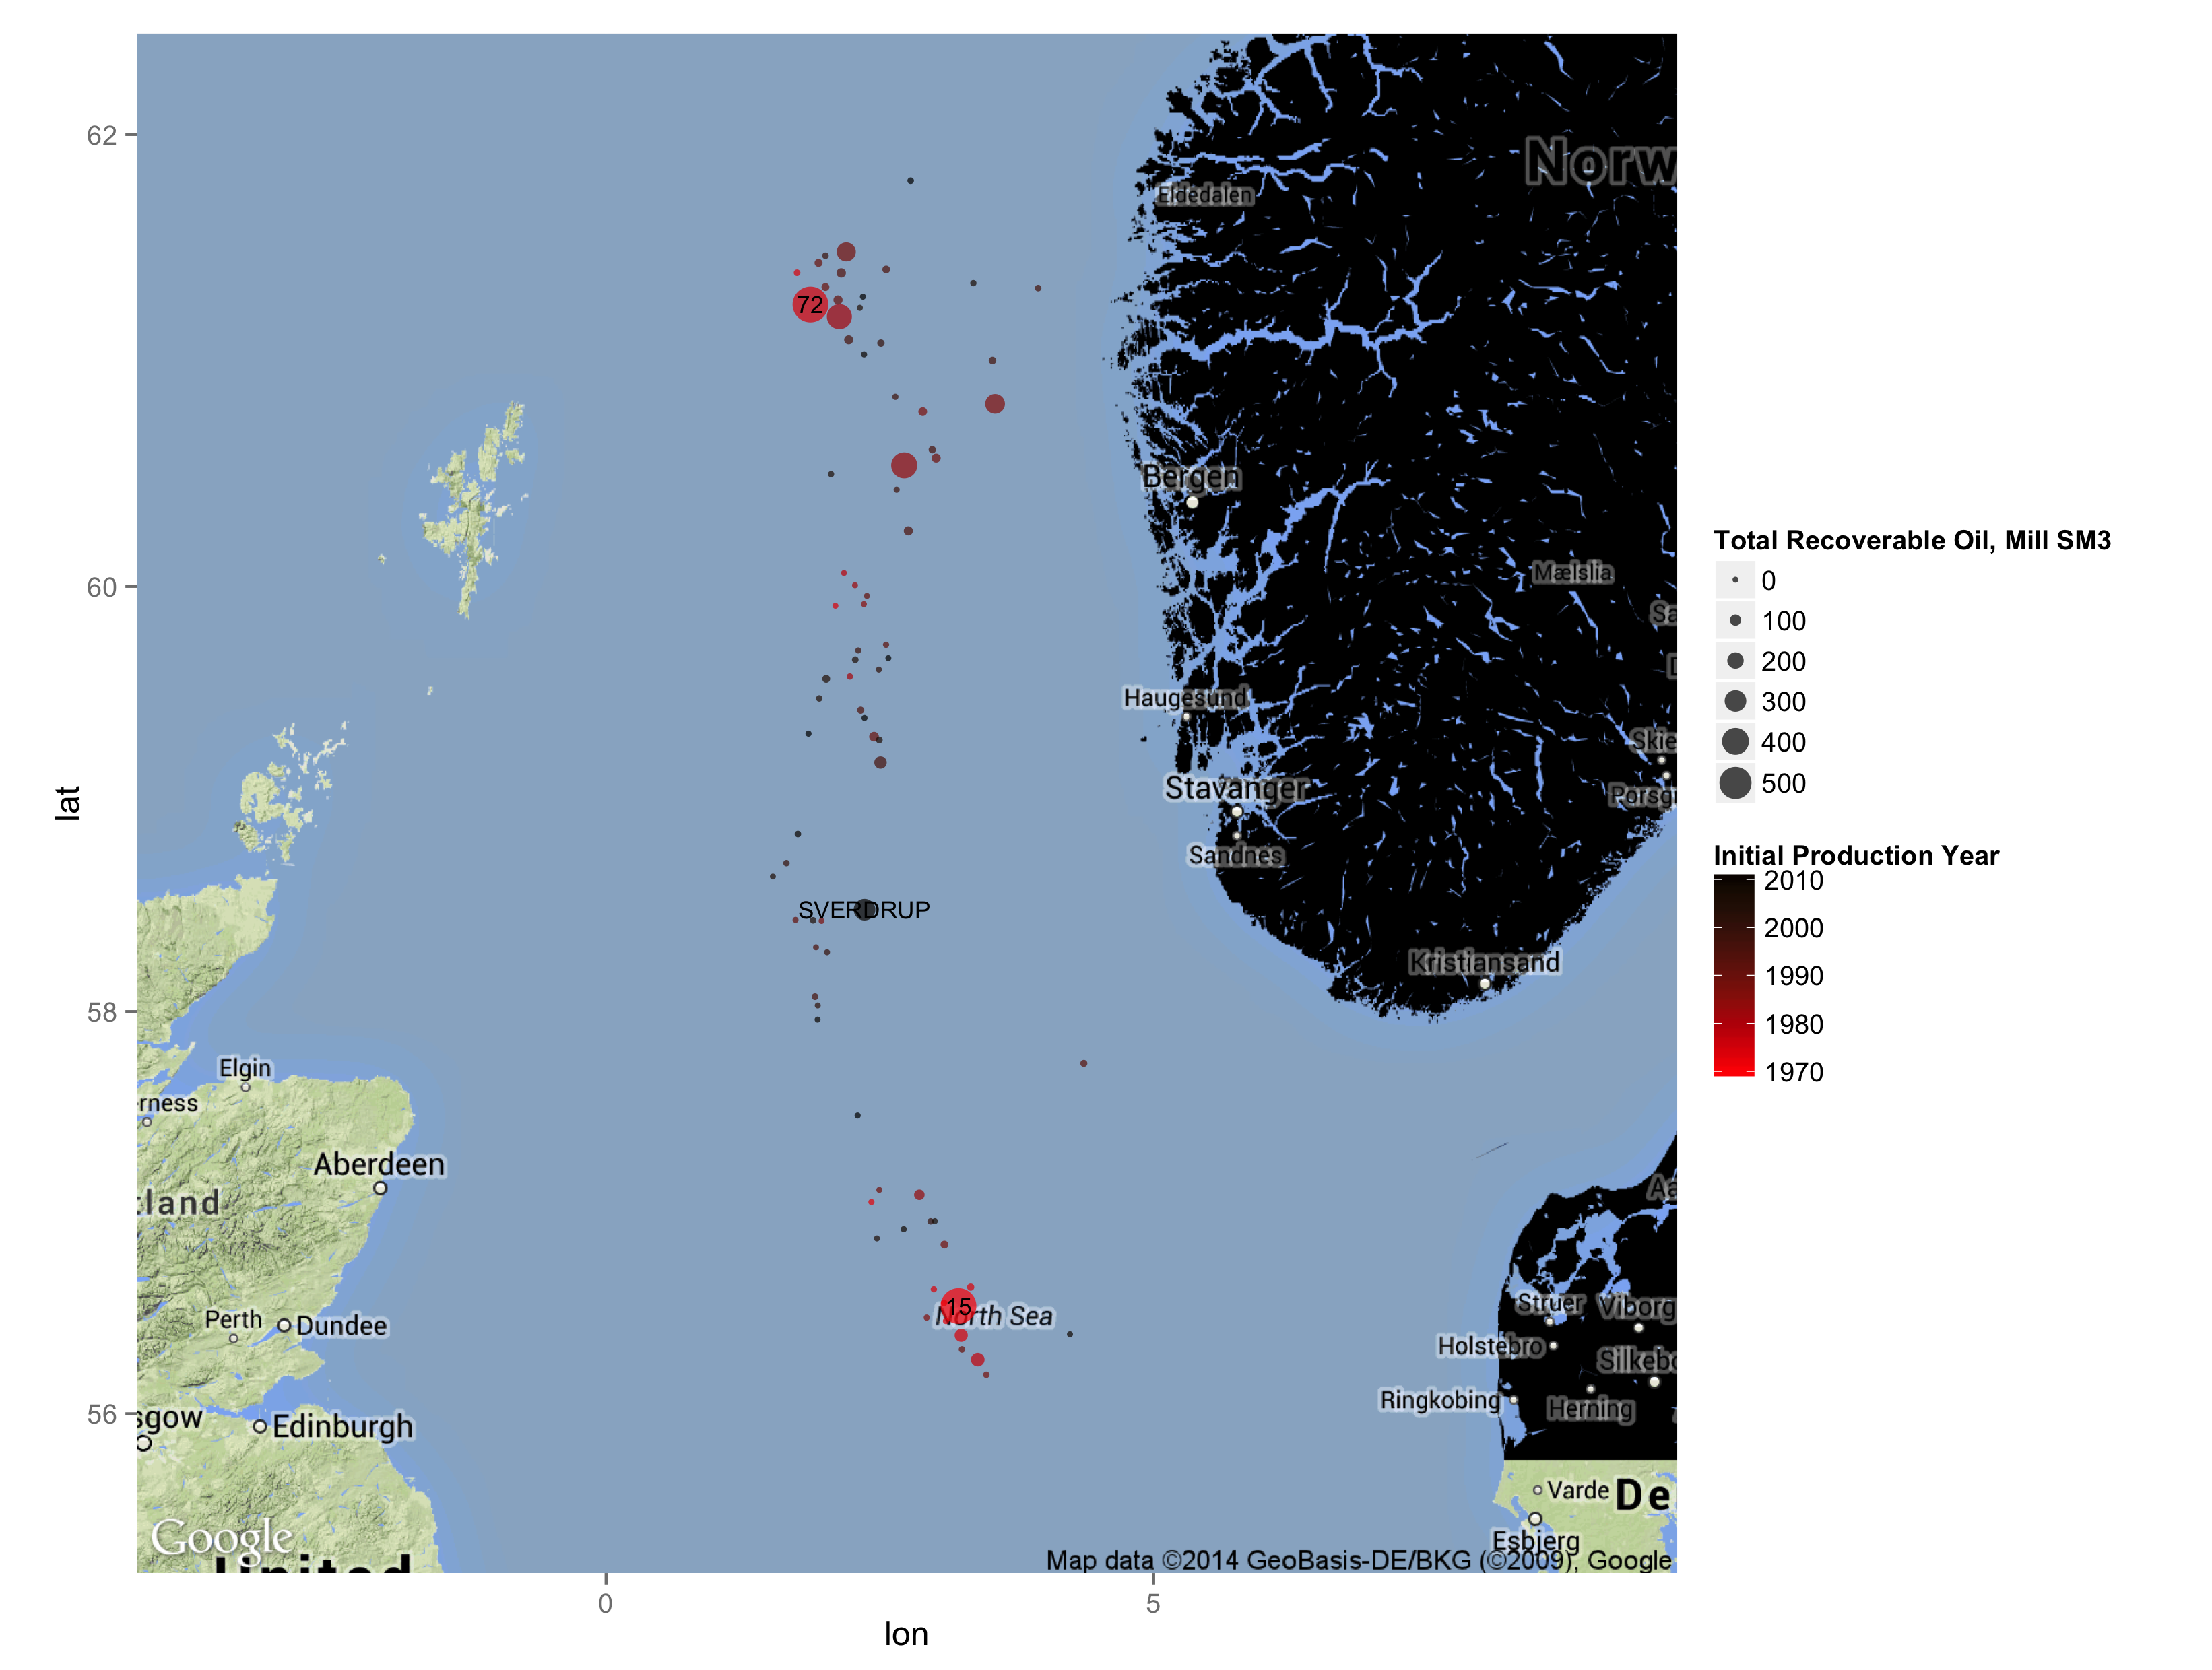
\includegraphics[width=.8\textwidth]{figures/north_sea_reserves.png}	
	\label{north_sea_reserves}
	\end{figure}
\end{frame}


\begin{frame}[plain]
	\begin{figure}
	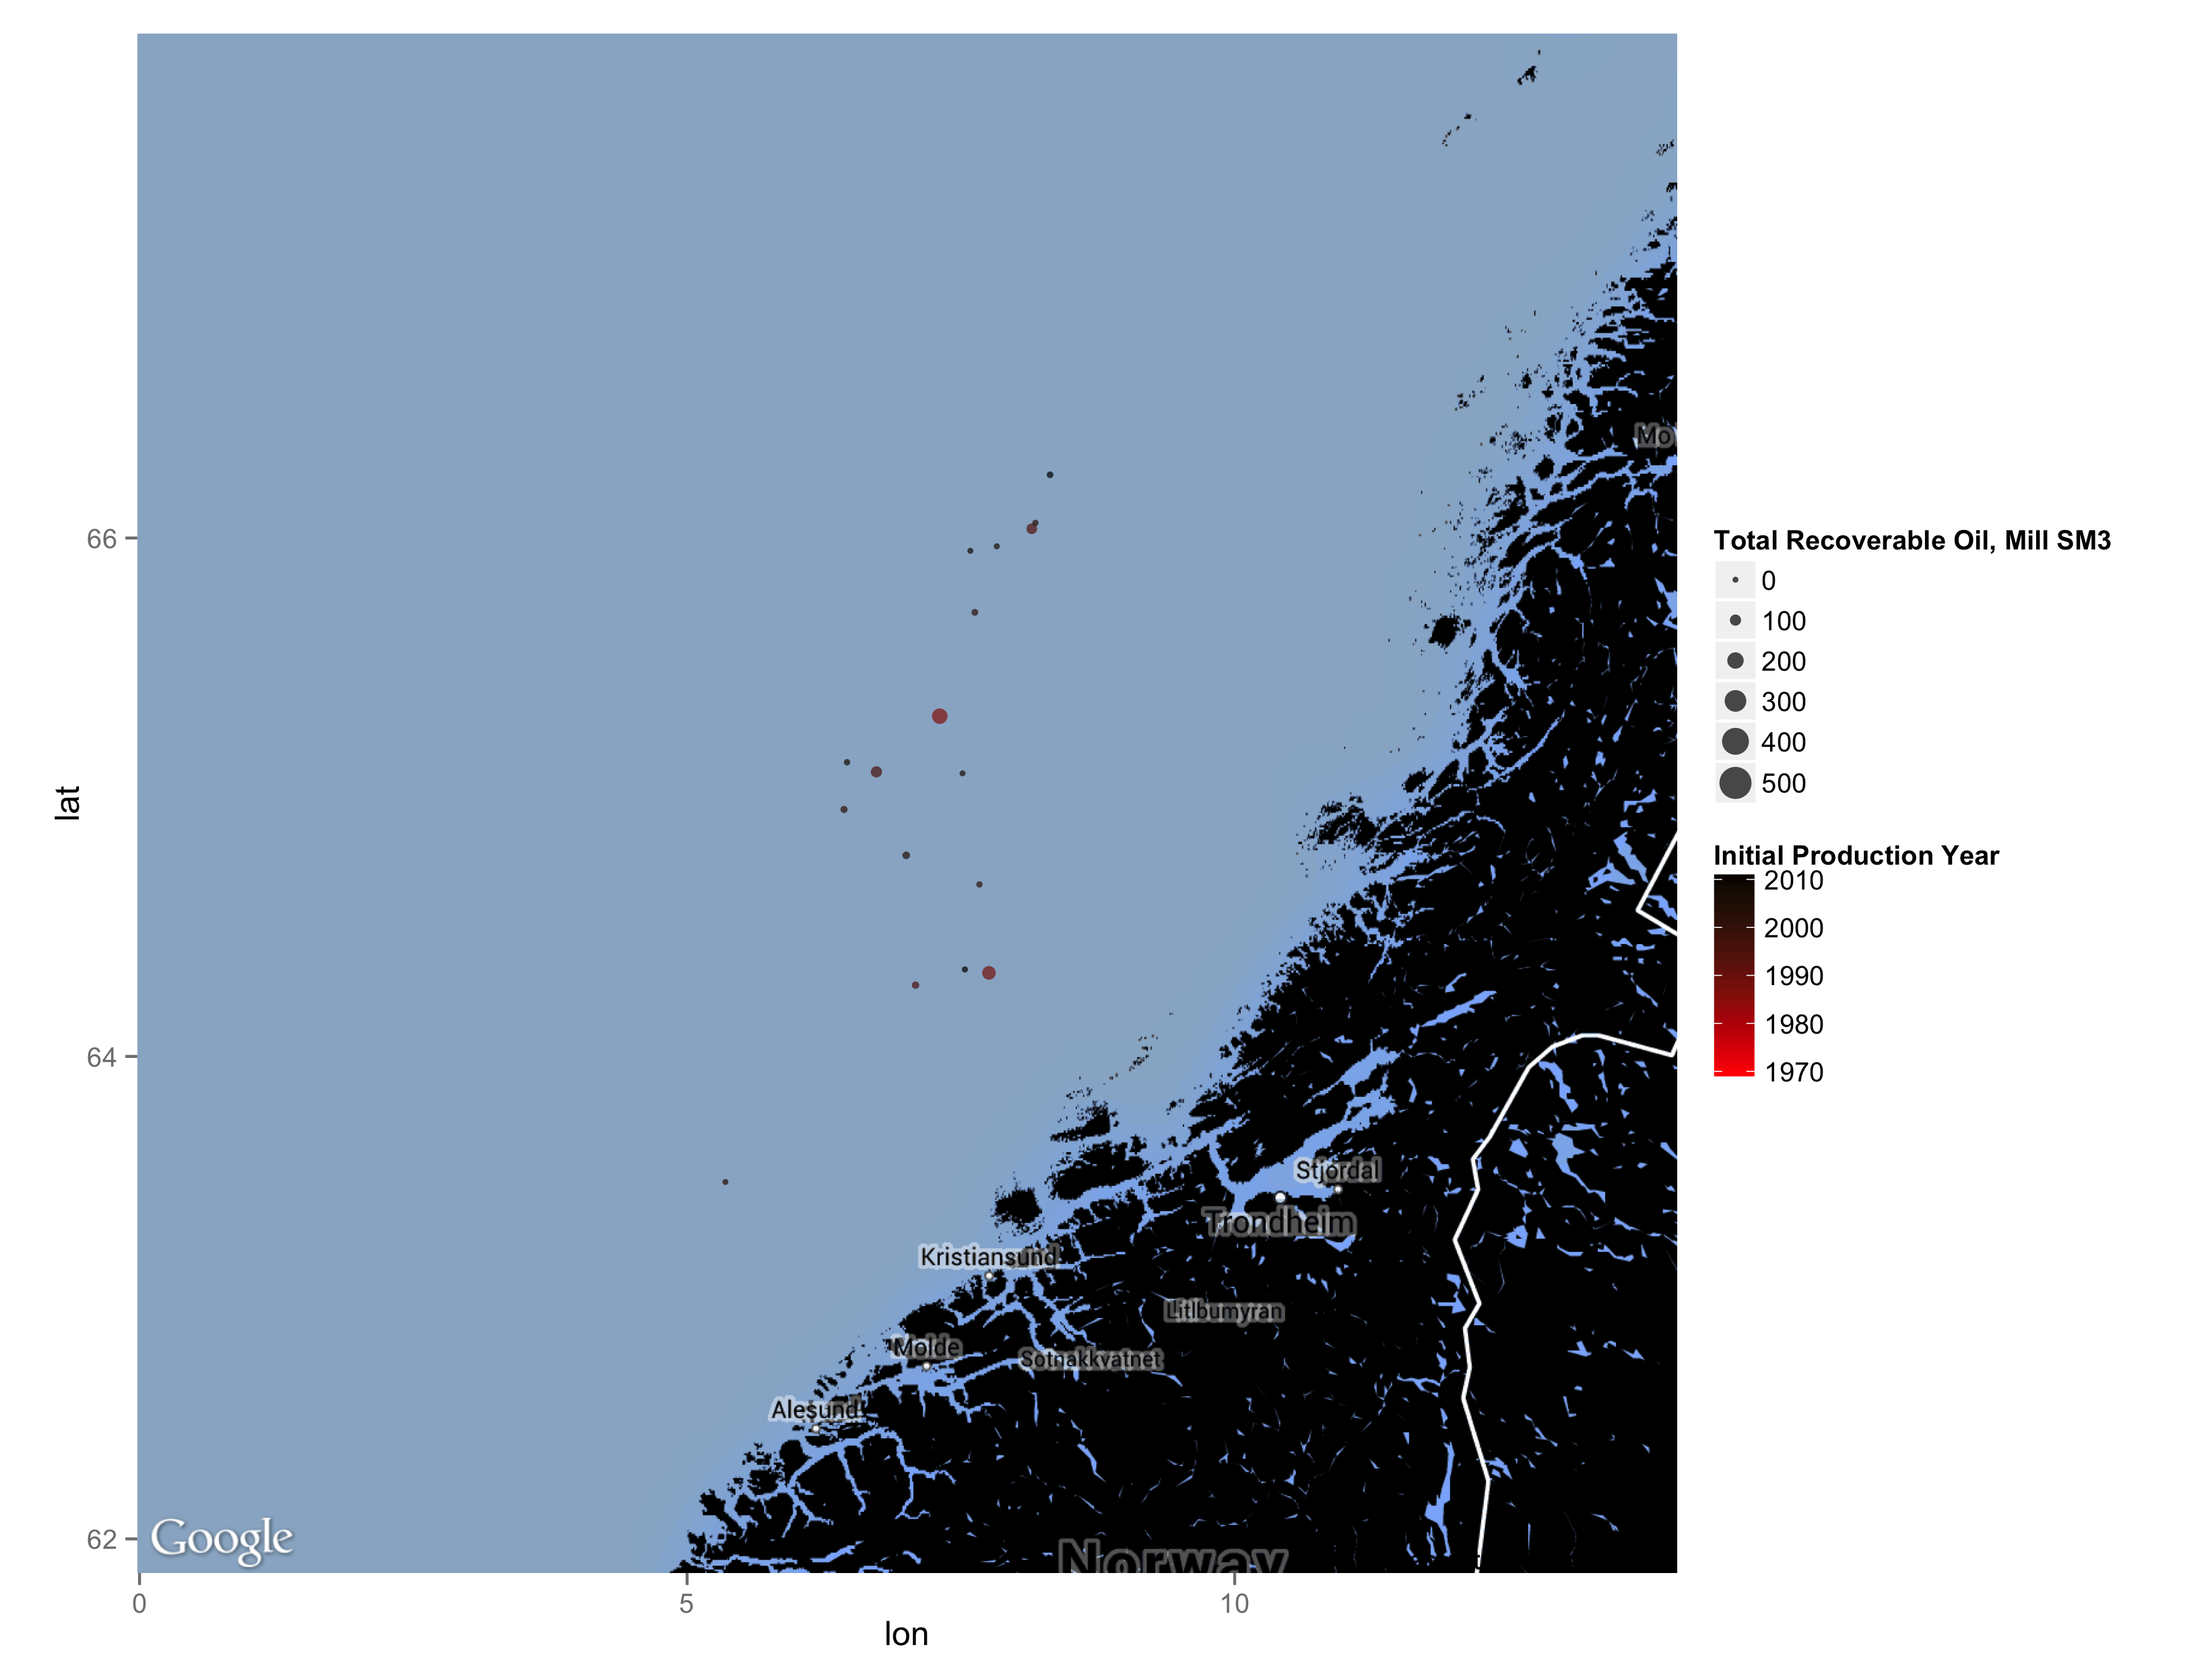
\includegraphics[width=.8\textwidth]{figures/norwegian_sea_reserves.png}
	
	\label{norwegian_sea_reserves}
	\end{figure}
\end{frame}


\begin{frame}[plain]

\begin{figure}
	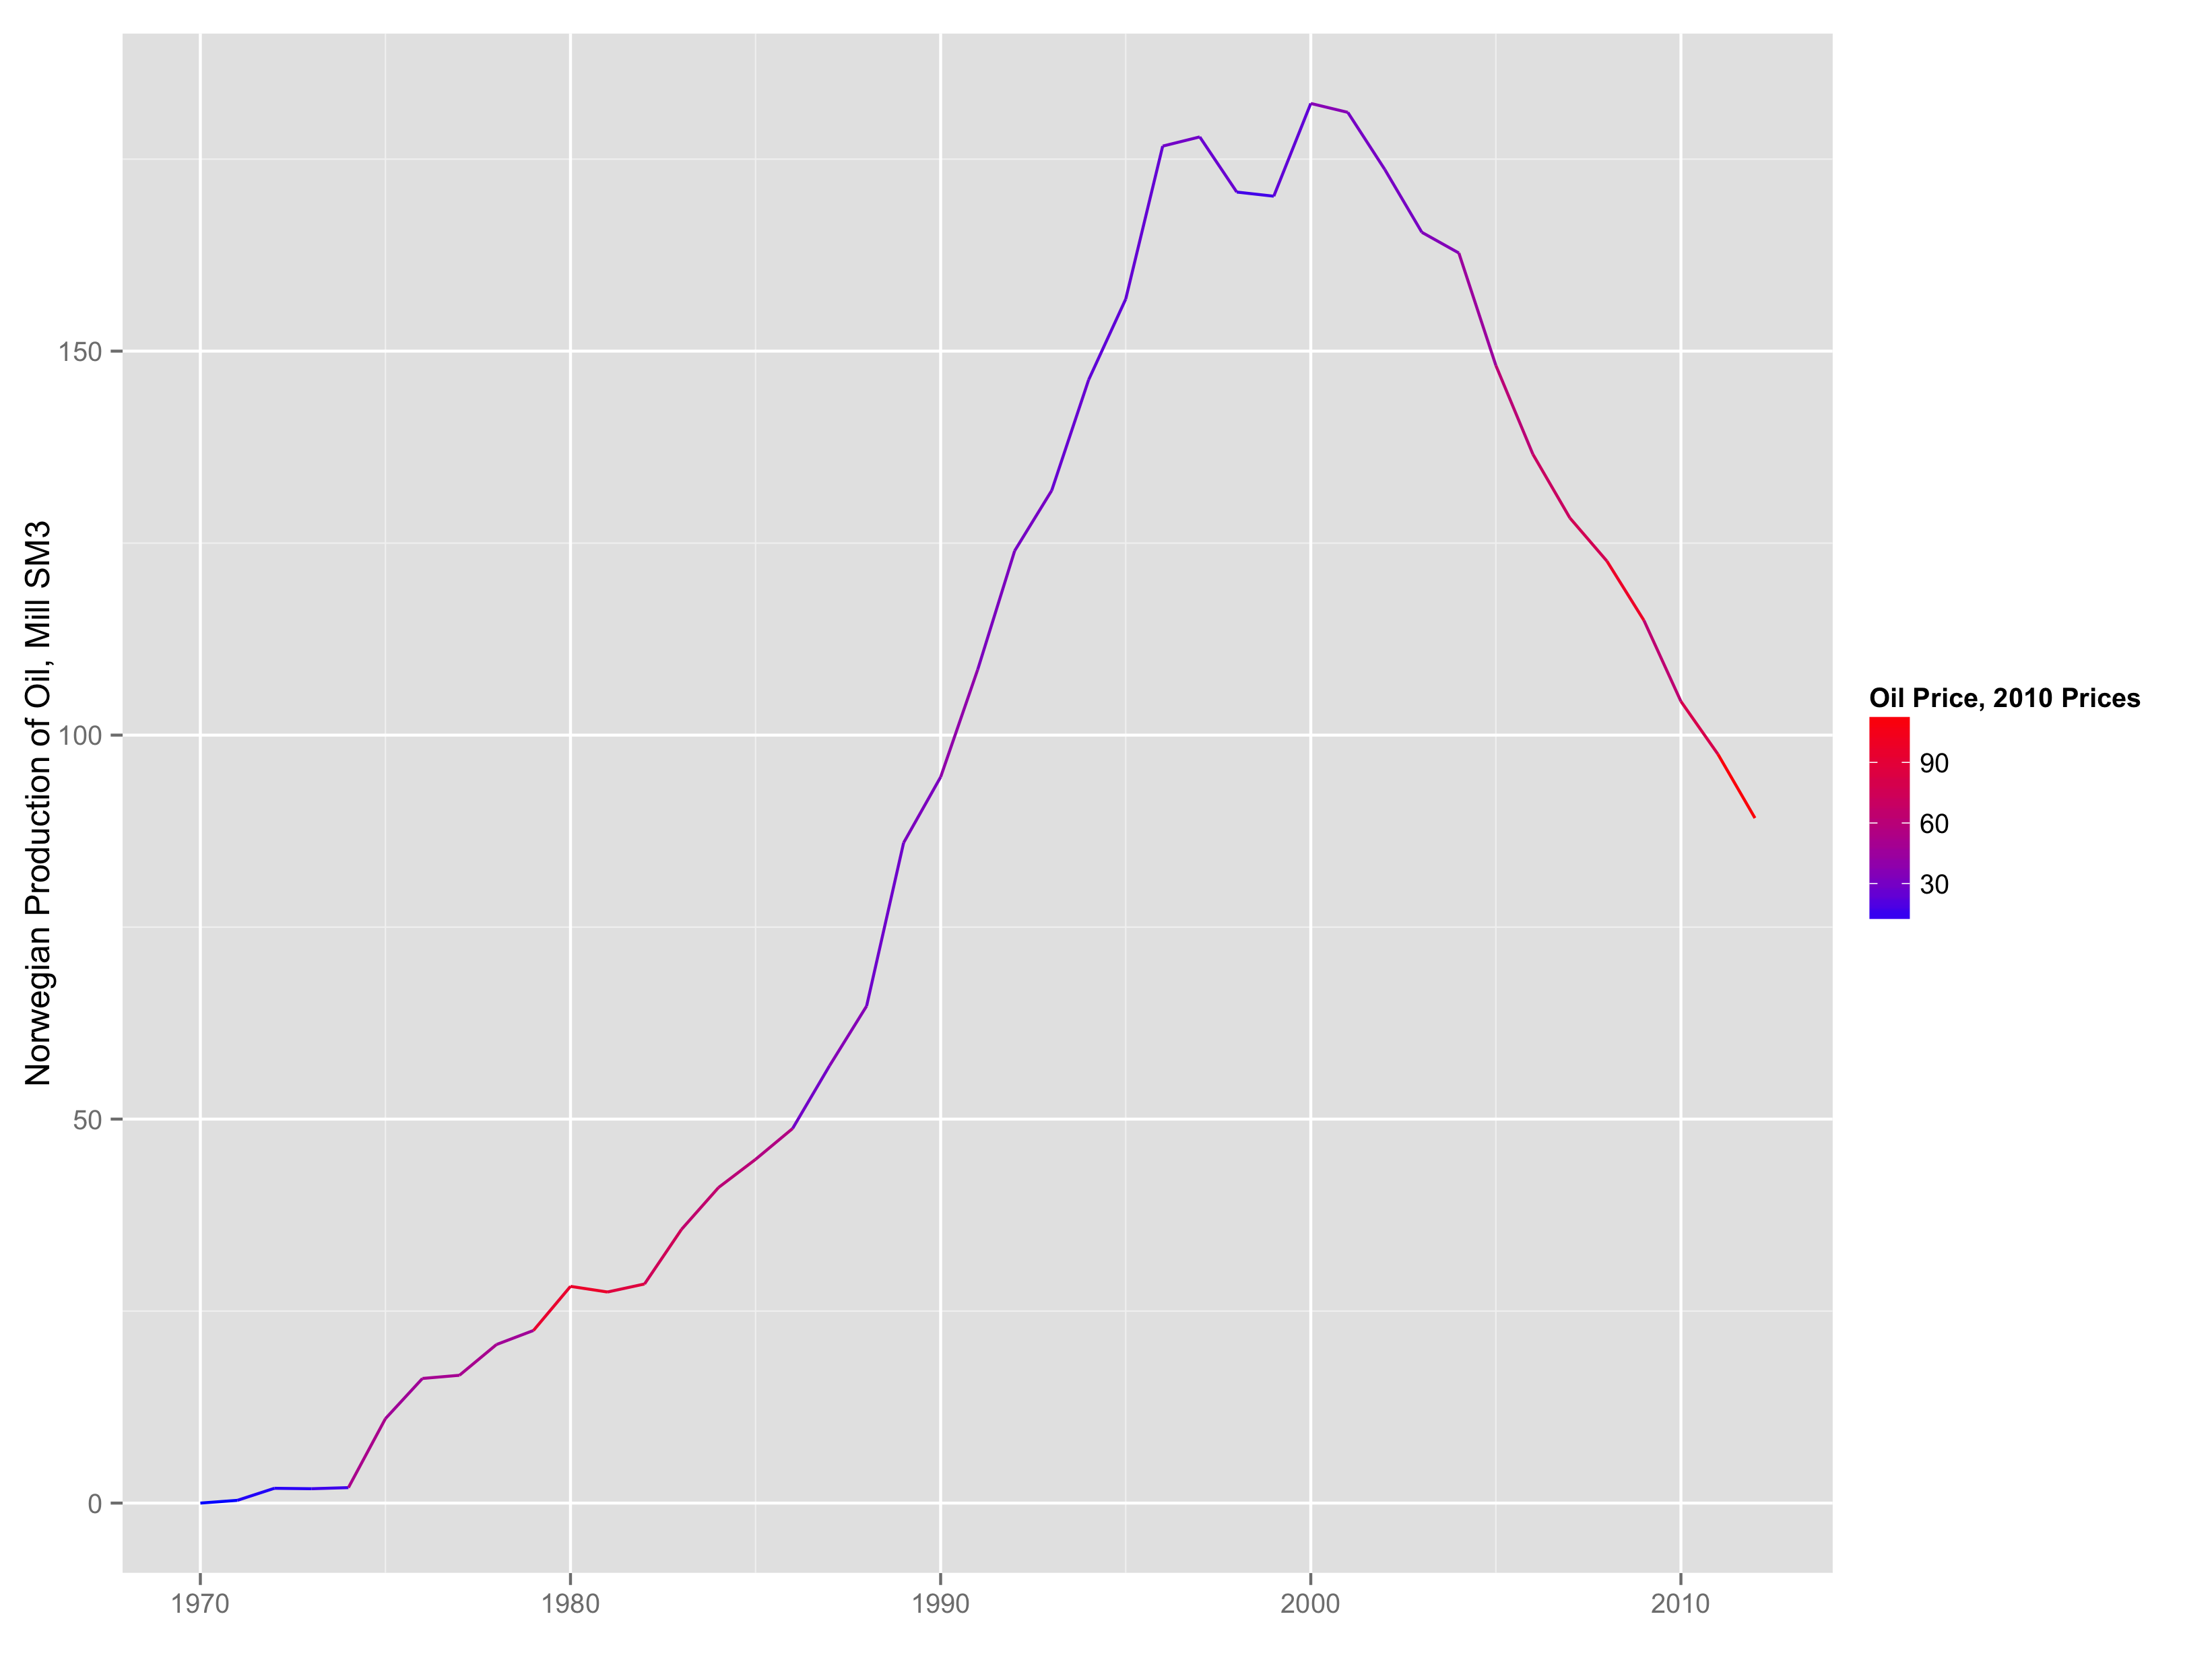
\includegraphics[width=.8\textwidth]{figures/oil_decline.png}
	
	\label{oil_decline}
\end{figure}

\end{frame}


\begin{frame}[plain]
	\begin{figure}
	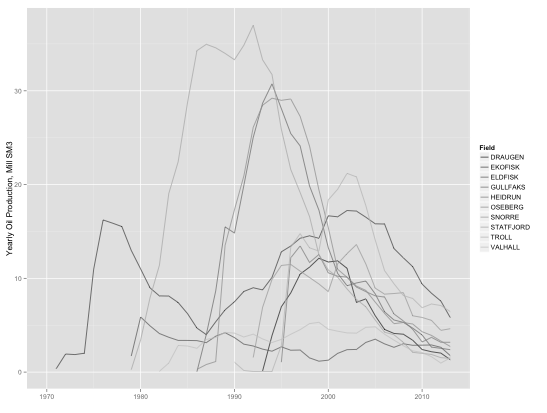
\includegraphics[width=.8\textwidth]{figures/top10_production.png}
	
	\label{top10_production}	
	\end{figure}
\end{frame}



\begin{frame}[plain]
	\begin{equation}
		\begin{split}
		 Log(Production_{i,t}) & = \alpha_0 + \alpha_1 time\_to\_peak_{i,t} + \alpha_2 time\_to\_peak_{i,t}^2 \\
		& \quad + \alpha_3 time\_to\_peak_{i,t}^3  + \alpha_4 peak\_to\_end_{i,t} + \alpha_5 peak\_to\_end_{i,t}^2 \\
		& \quad + \alpha_6 peak\_to\_end_{i,t}^3 + \gamma total\_recoverable\_oil_i \\
		& \quad + \beta_1 oil\_price + \beta_2 oil\_price\_l1 + ...+ \epsilon
		\end{split}
	\label{glm_eqn}
		\end{equation}
\end{frame}


\begin{frame}[plain]
	\begin{figure}
	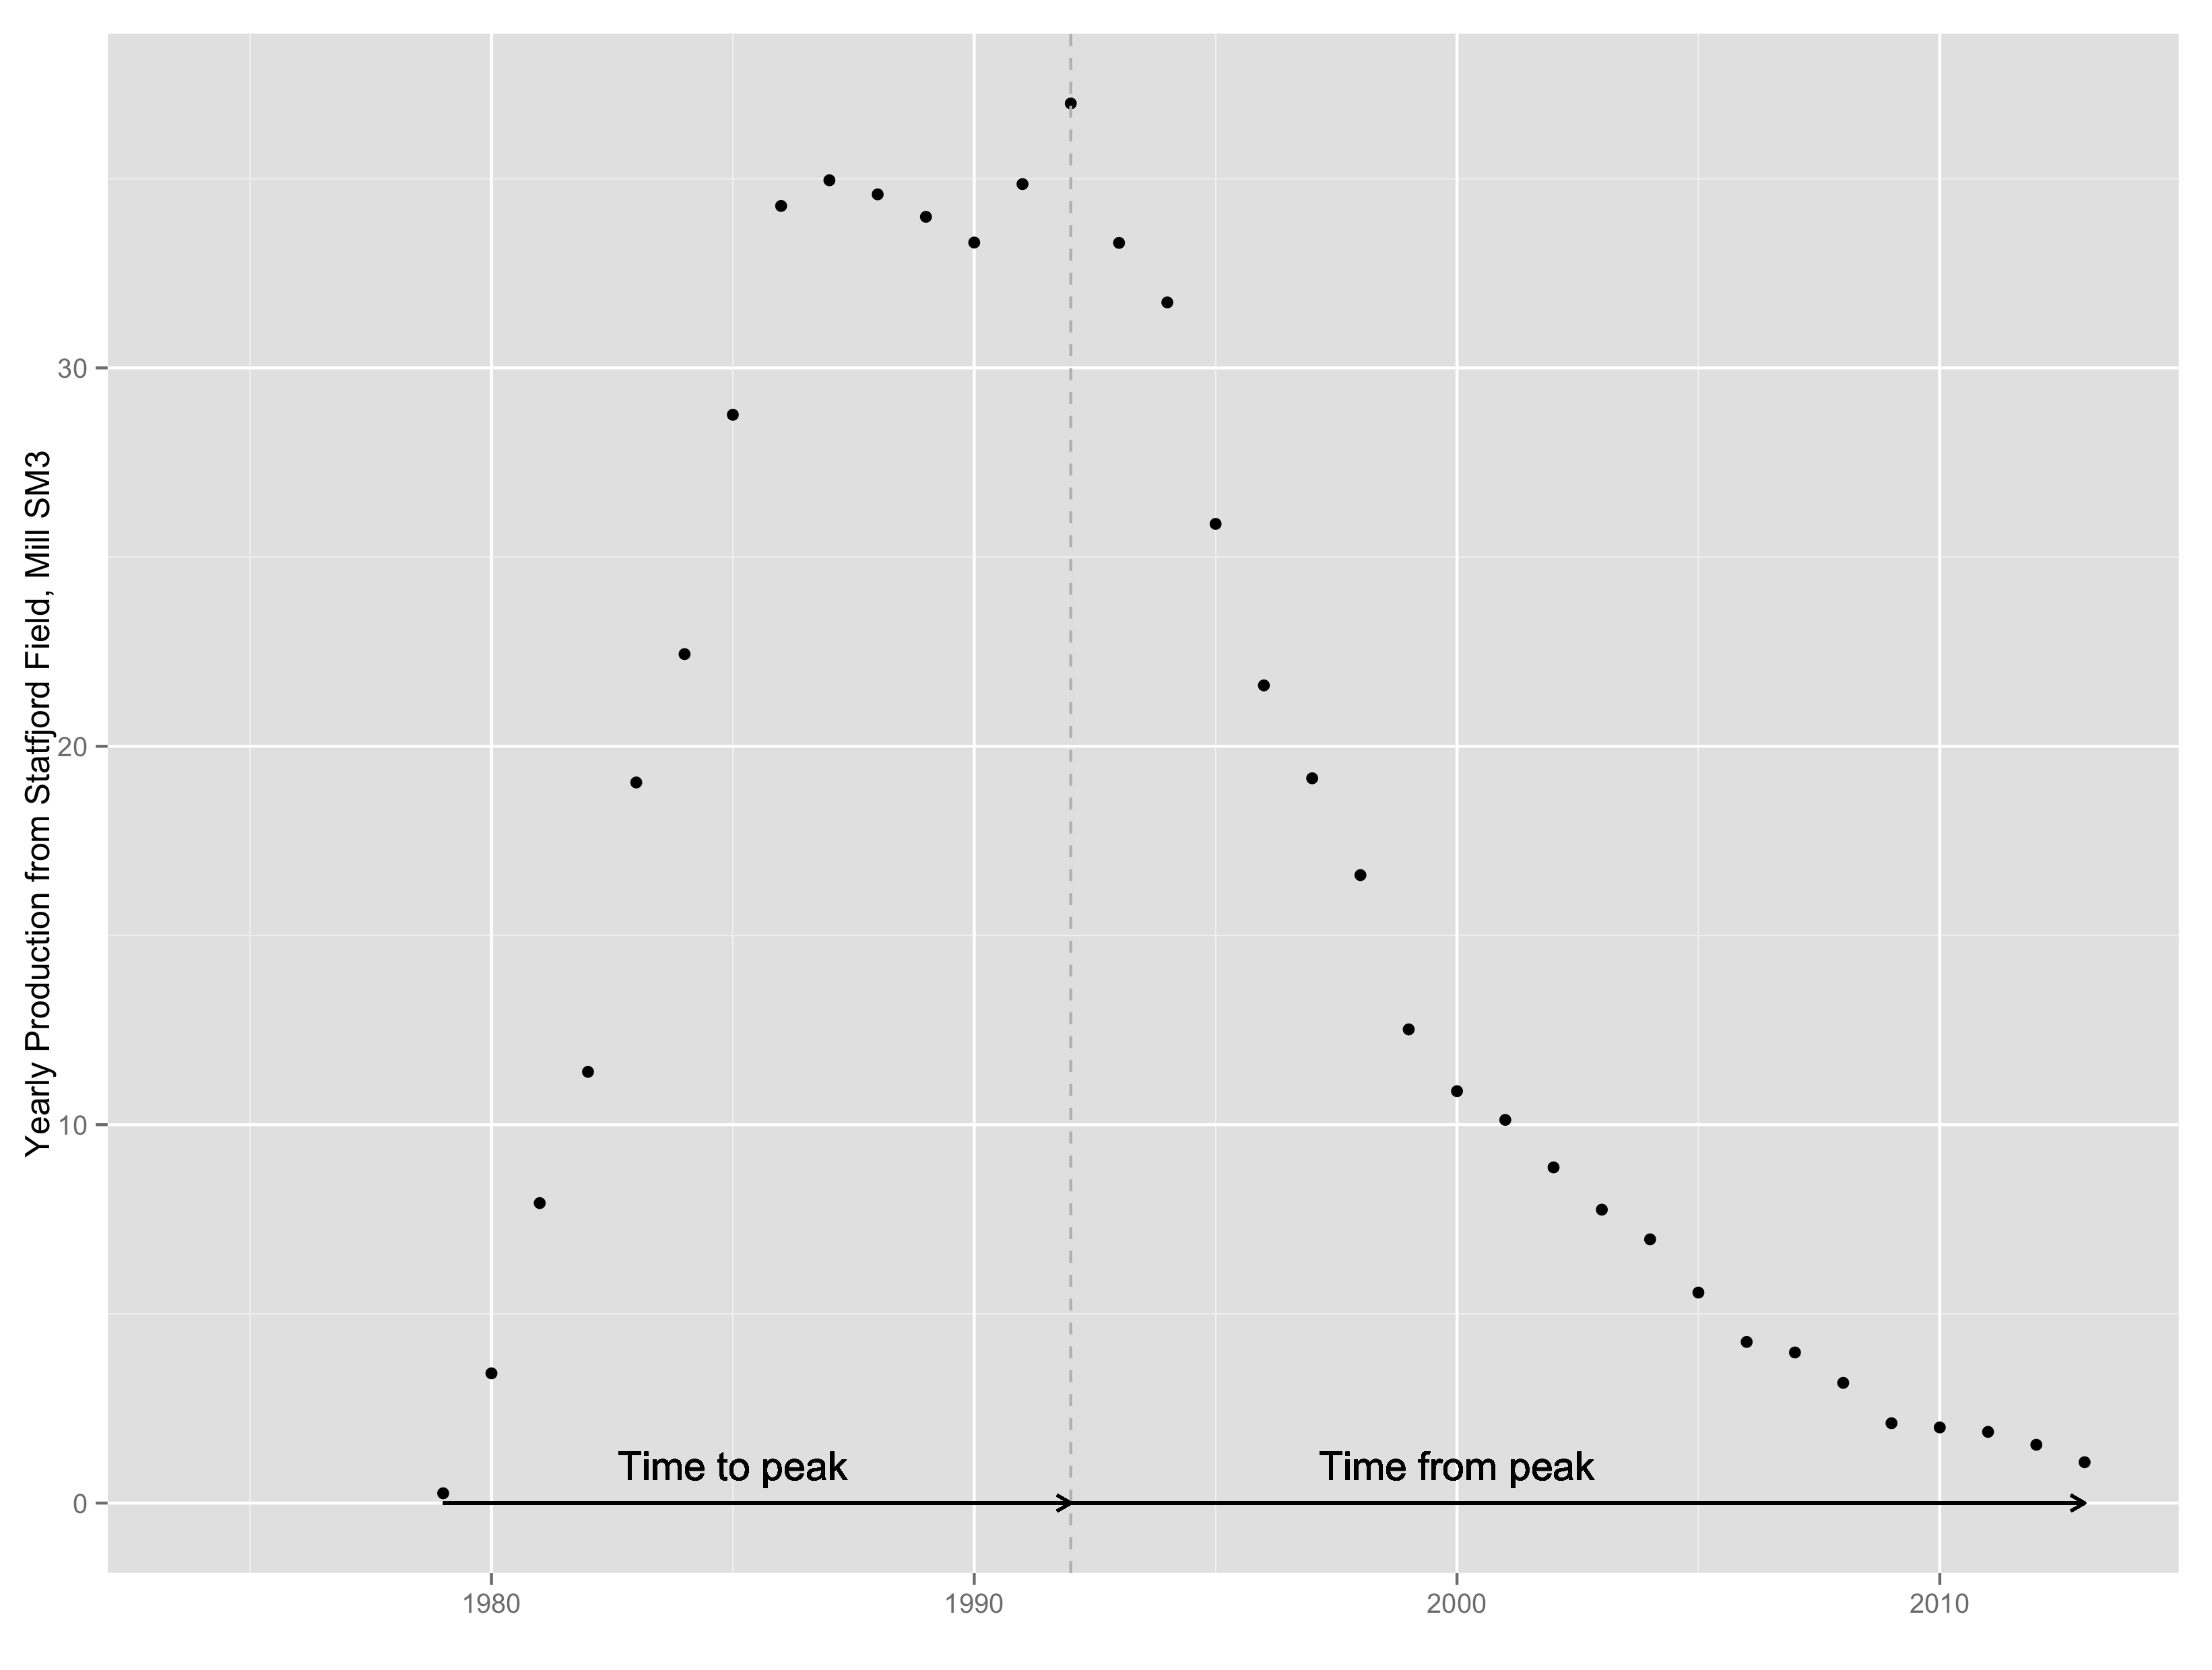
\includegraphics[width=.8\textwidth]{figures/statfjord_dem.png}
	
	\label{statfjord_dem}
	\end{figure}
\end{frame}


\begin{frame}[plain]
	\begin{figure}
	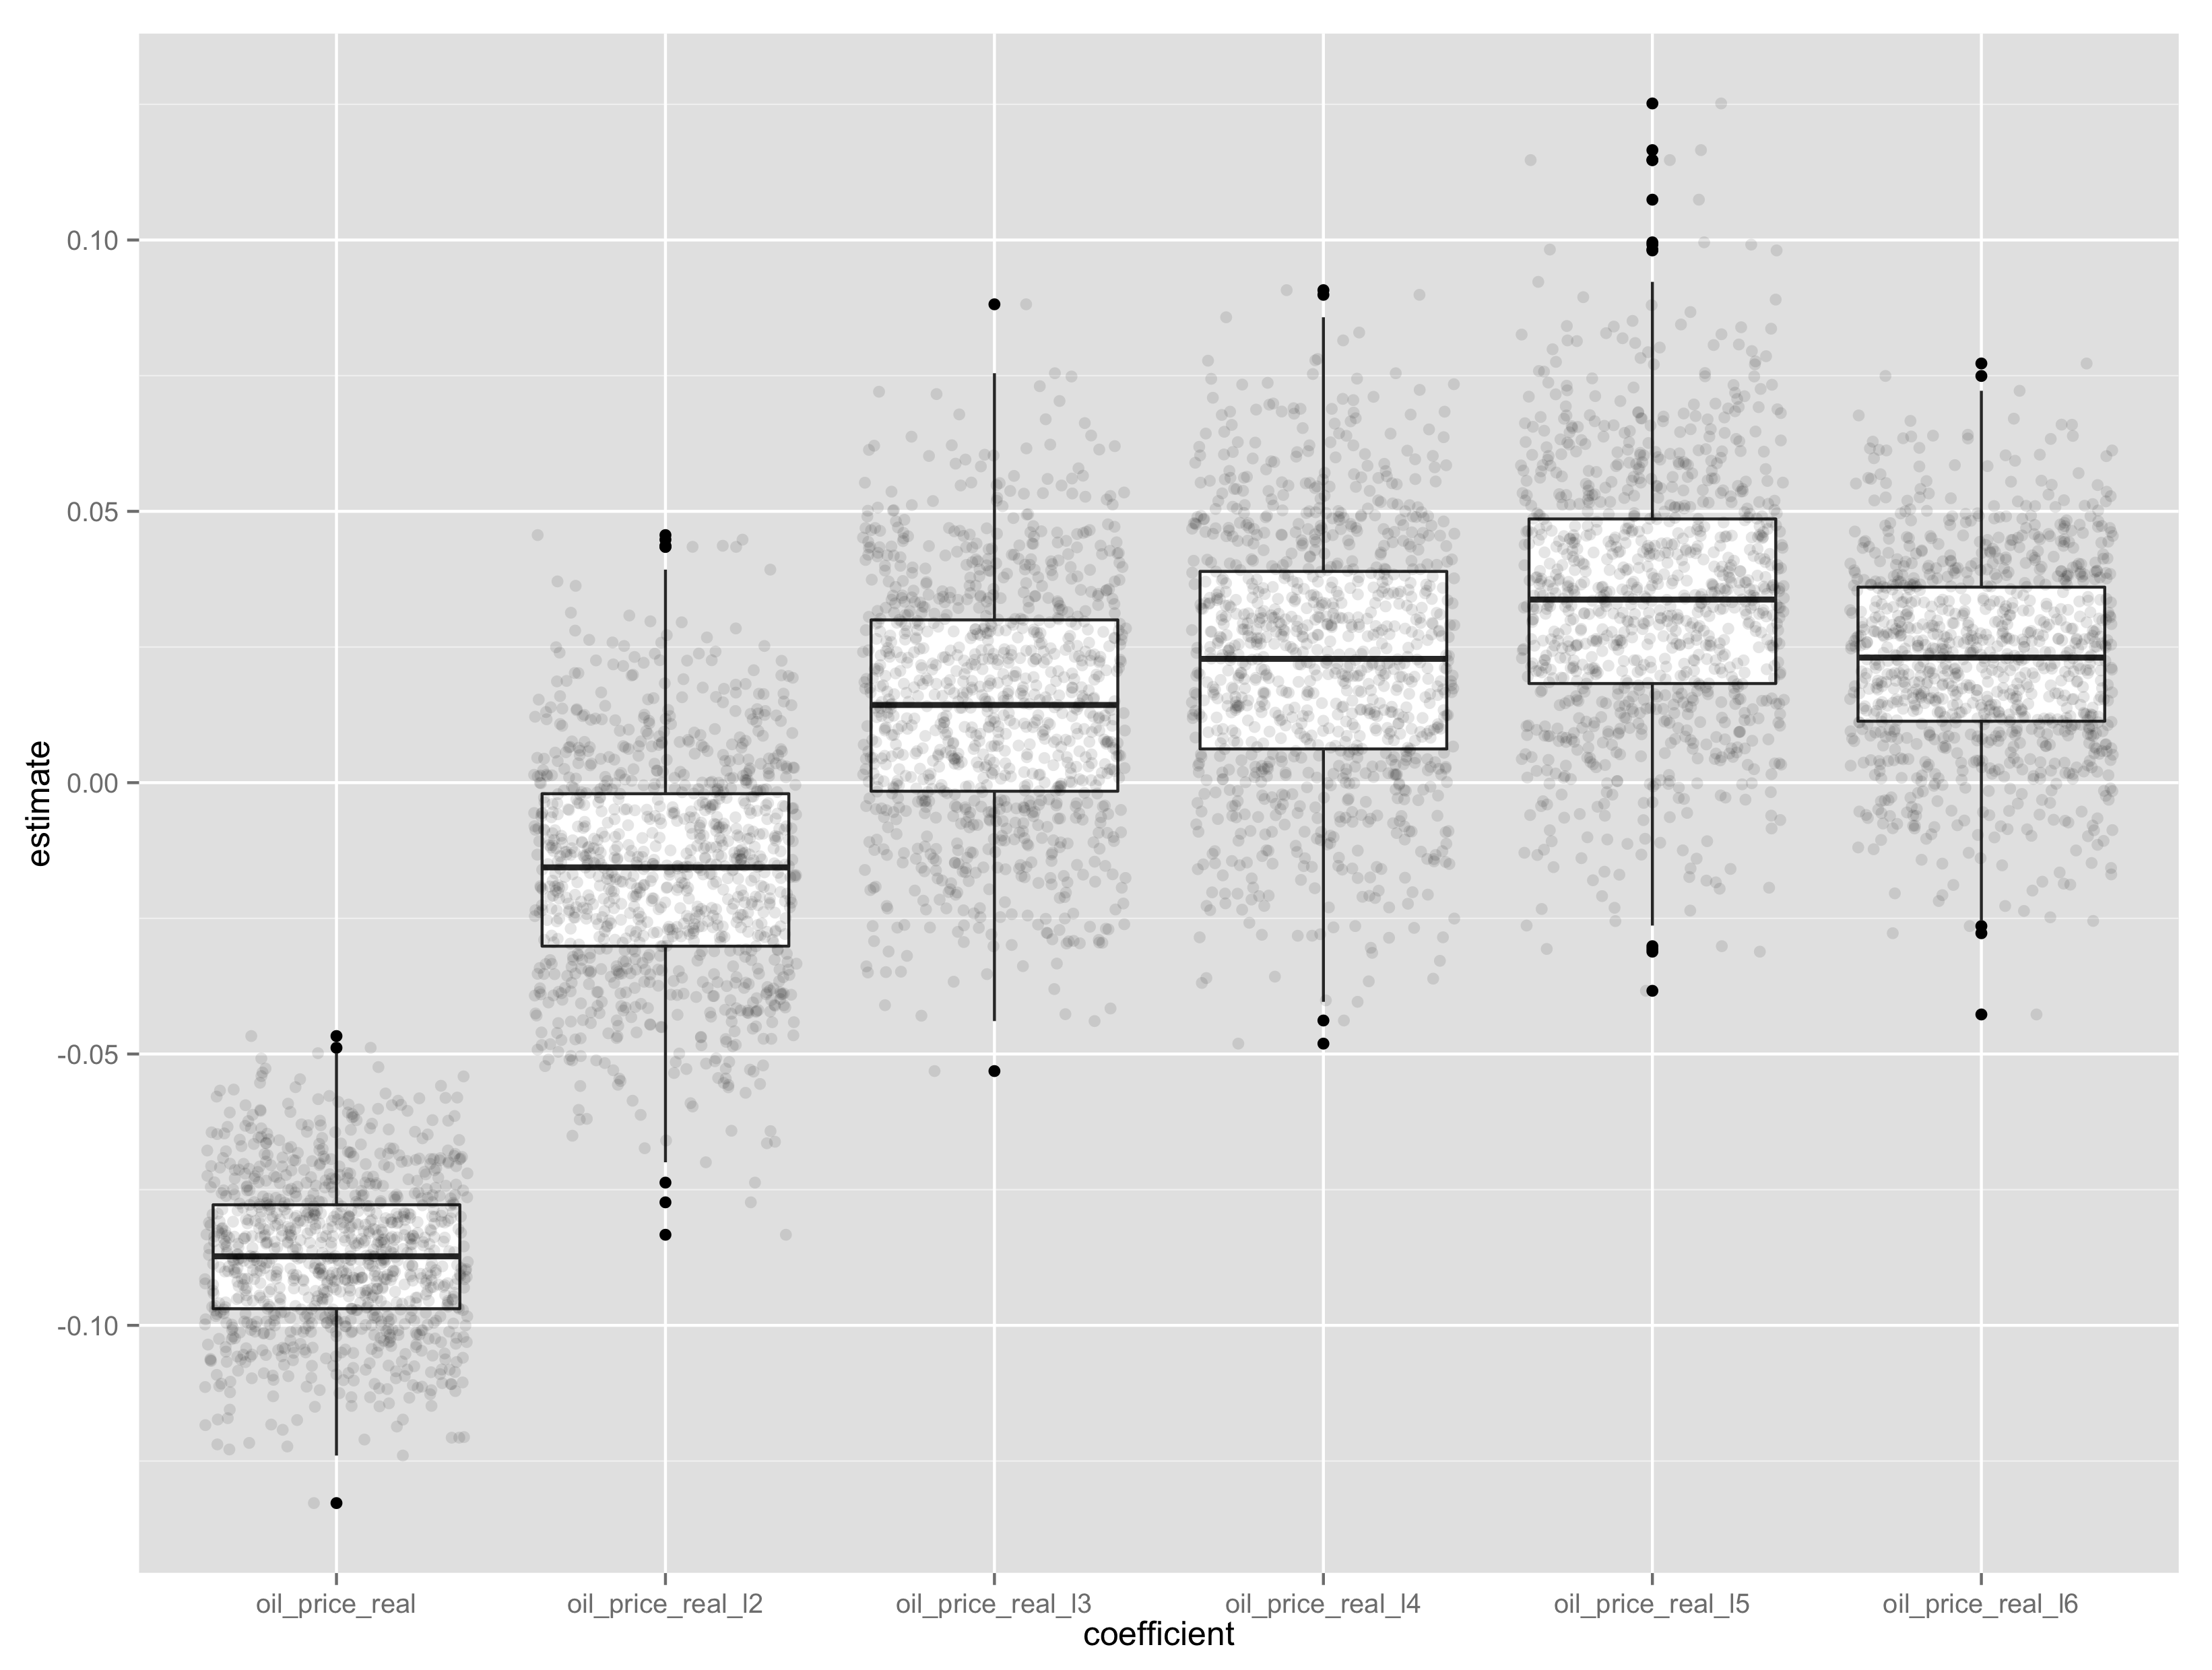
\includegraphics[width=.8\textwidth]{figures/glm_dirty_box.png}
	
	\label{glm_dirty_box}
	\end{figure}
\end{frame}


\begin{frame}[plain]
	\begin{equation}
	Production_{t}=f(time) + \epsilon
		\label{simp_eqn}
	\end{equation}
\end{frame}


\begin{frame}[plain]
	\begin{figure}
		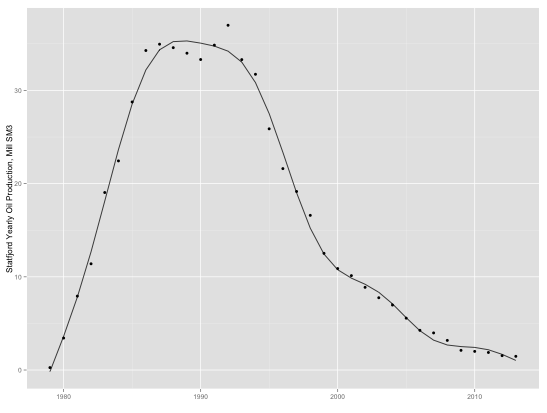
\includegraphics[width=.8\textwidth]{figures/statfjord_gam.png}
		
		\label{statfjord_gam}
	\end{figure}
\end{frame}


\begin{frame}[plain]
	\begin{equation}
	\begin{split}
		Log(Production_{i,t})&=f(time\_to\_peak_{i,t}, total\_recoverable\_oil_i) \\
		& \quad + f(peak\_to\_end_{i,t}, total\_recoverable\_oil_i) \\
		& \quad + \beta_1 oil\_price + \beta_2 oil\_price\_l1 + ... +  \epsilon
	\end{split}
	\label{gam_price_eqn}
	\end{equation}
\end{frame}



\begin{frame}[plain]
	Thin Plate (Regression) Splines (Duchon 1977)
	\begin{equation}
	y_i = g(x_1, x_2)
	\end{equation}

	\begin{equation}
	\min \|\boldsymbol{y-f}\|^2 + \lambda J_{md}(f)
	\end{equation}

	\begin{equation}
	J_{22}{f}= \diffp[2]{f}{x_1}^2 + \diffp[2]{f}{{x_1}{x_2}} + \diffp[2]{f}{x_2}^2dx_1 dx_2
	\end{equation}
\end{frame}

\begin{frame}[plain]
	\begin{figure}
		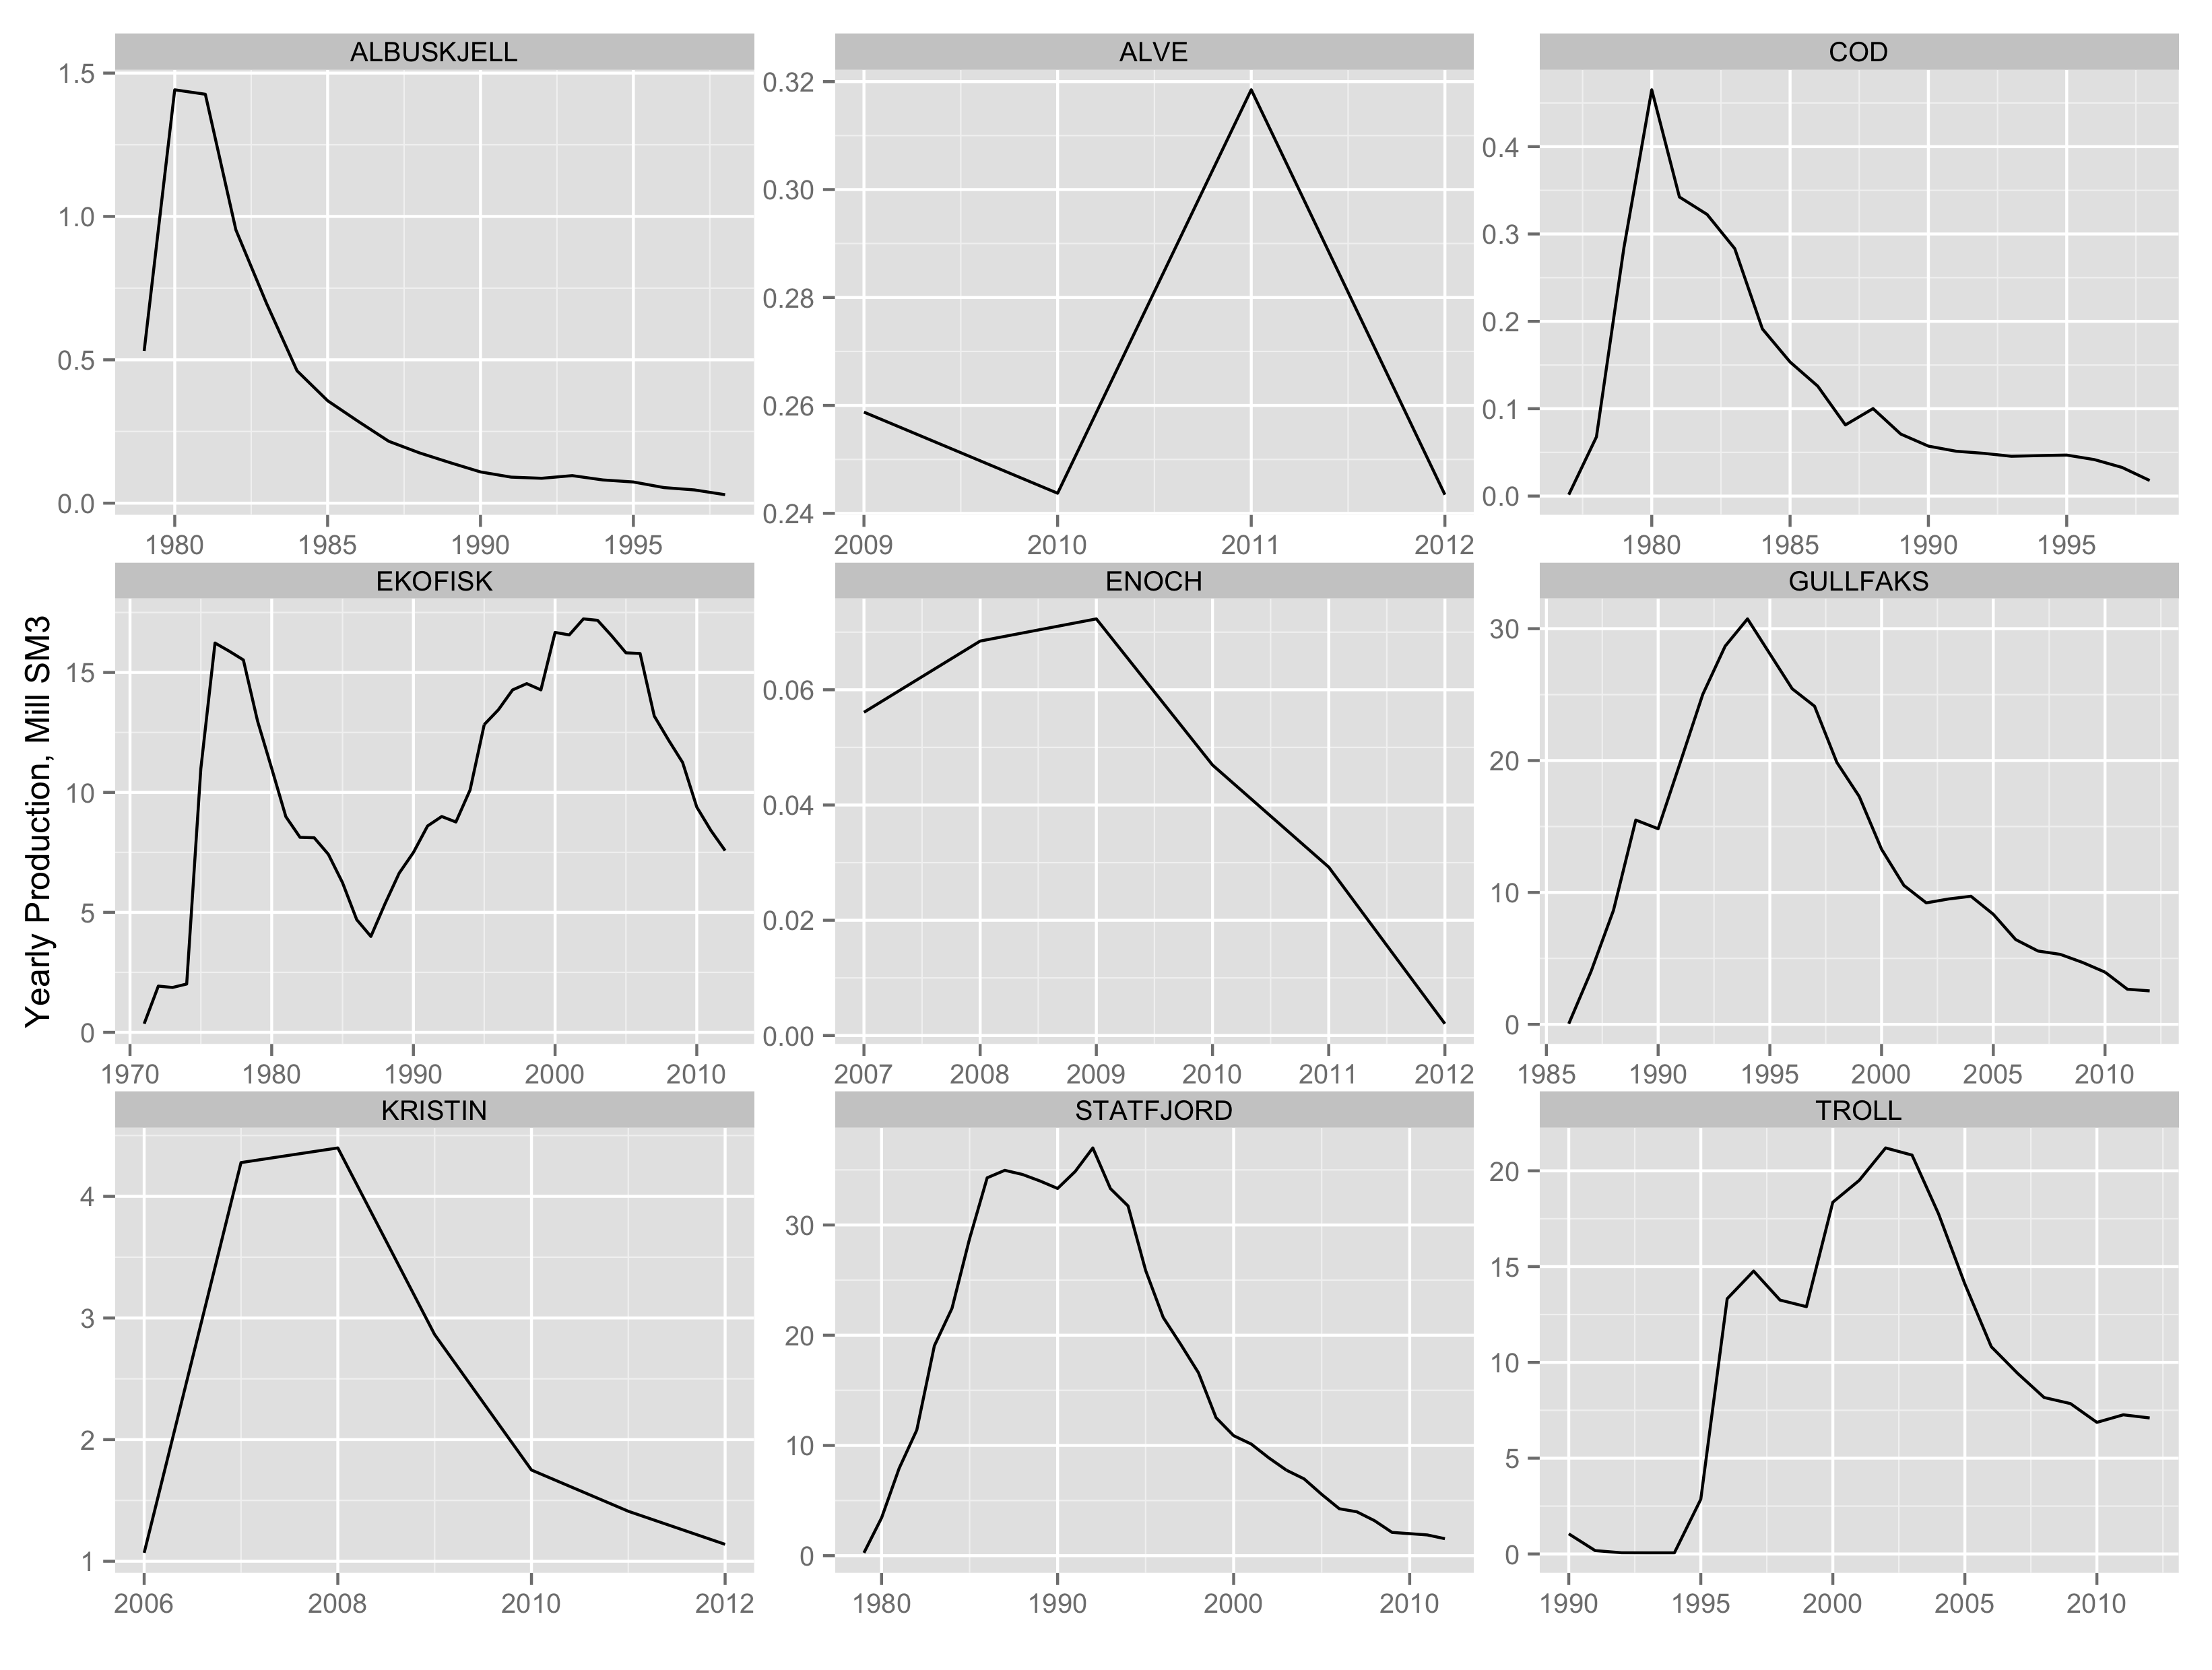
\includegraphics[width=.8\textwidth]{figures/field_inspection.png}
		
		\label{field_inspection}
	\end{figure}
\end{frame}


\begin{frame}[plain]
	\begin{figure}
		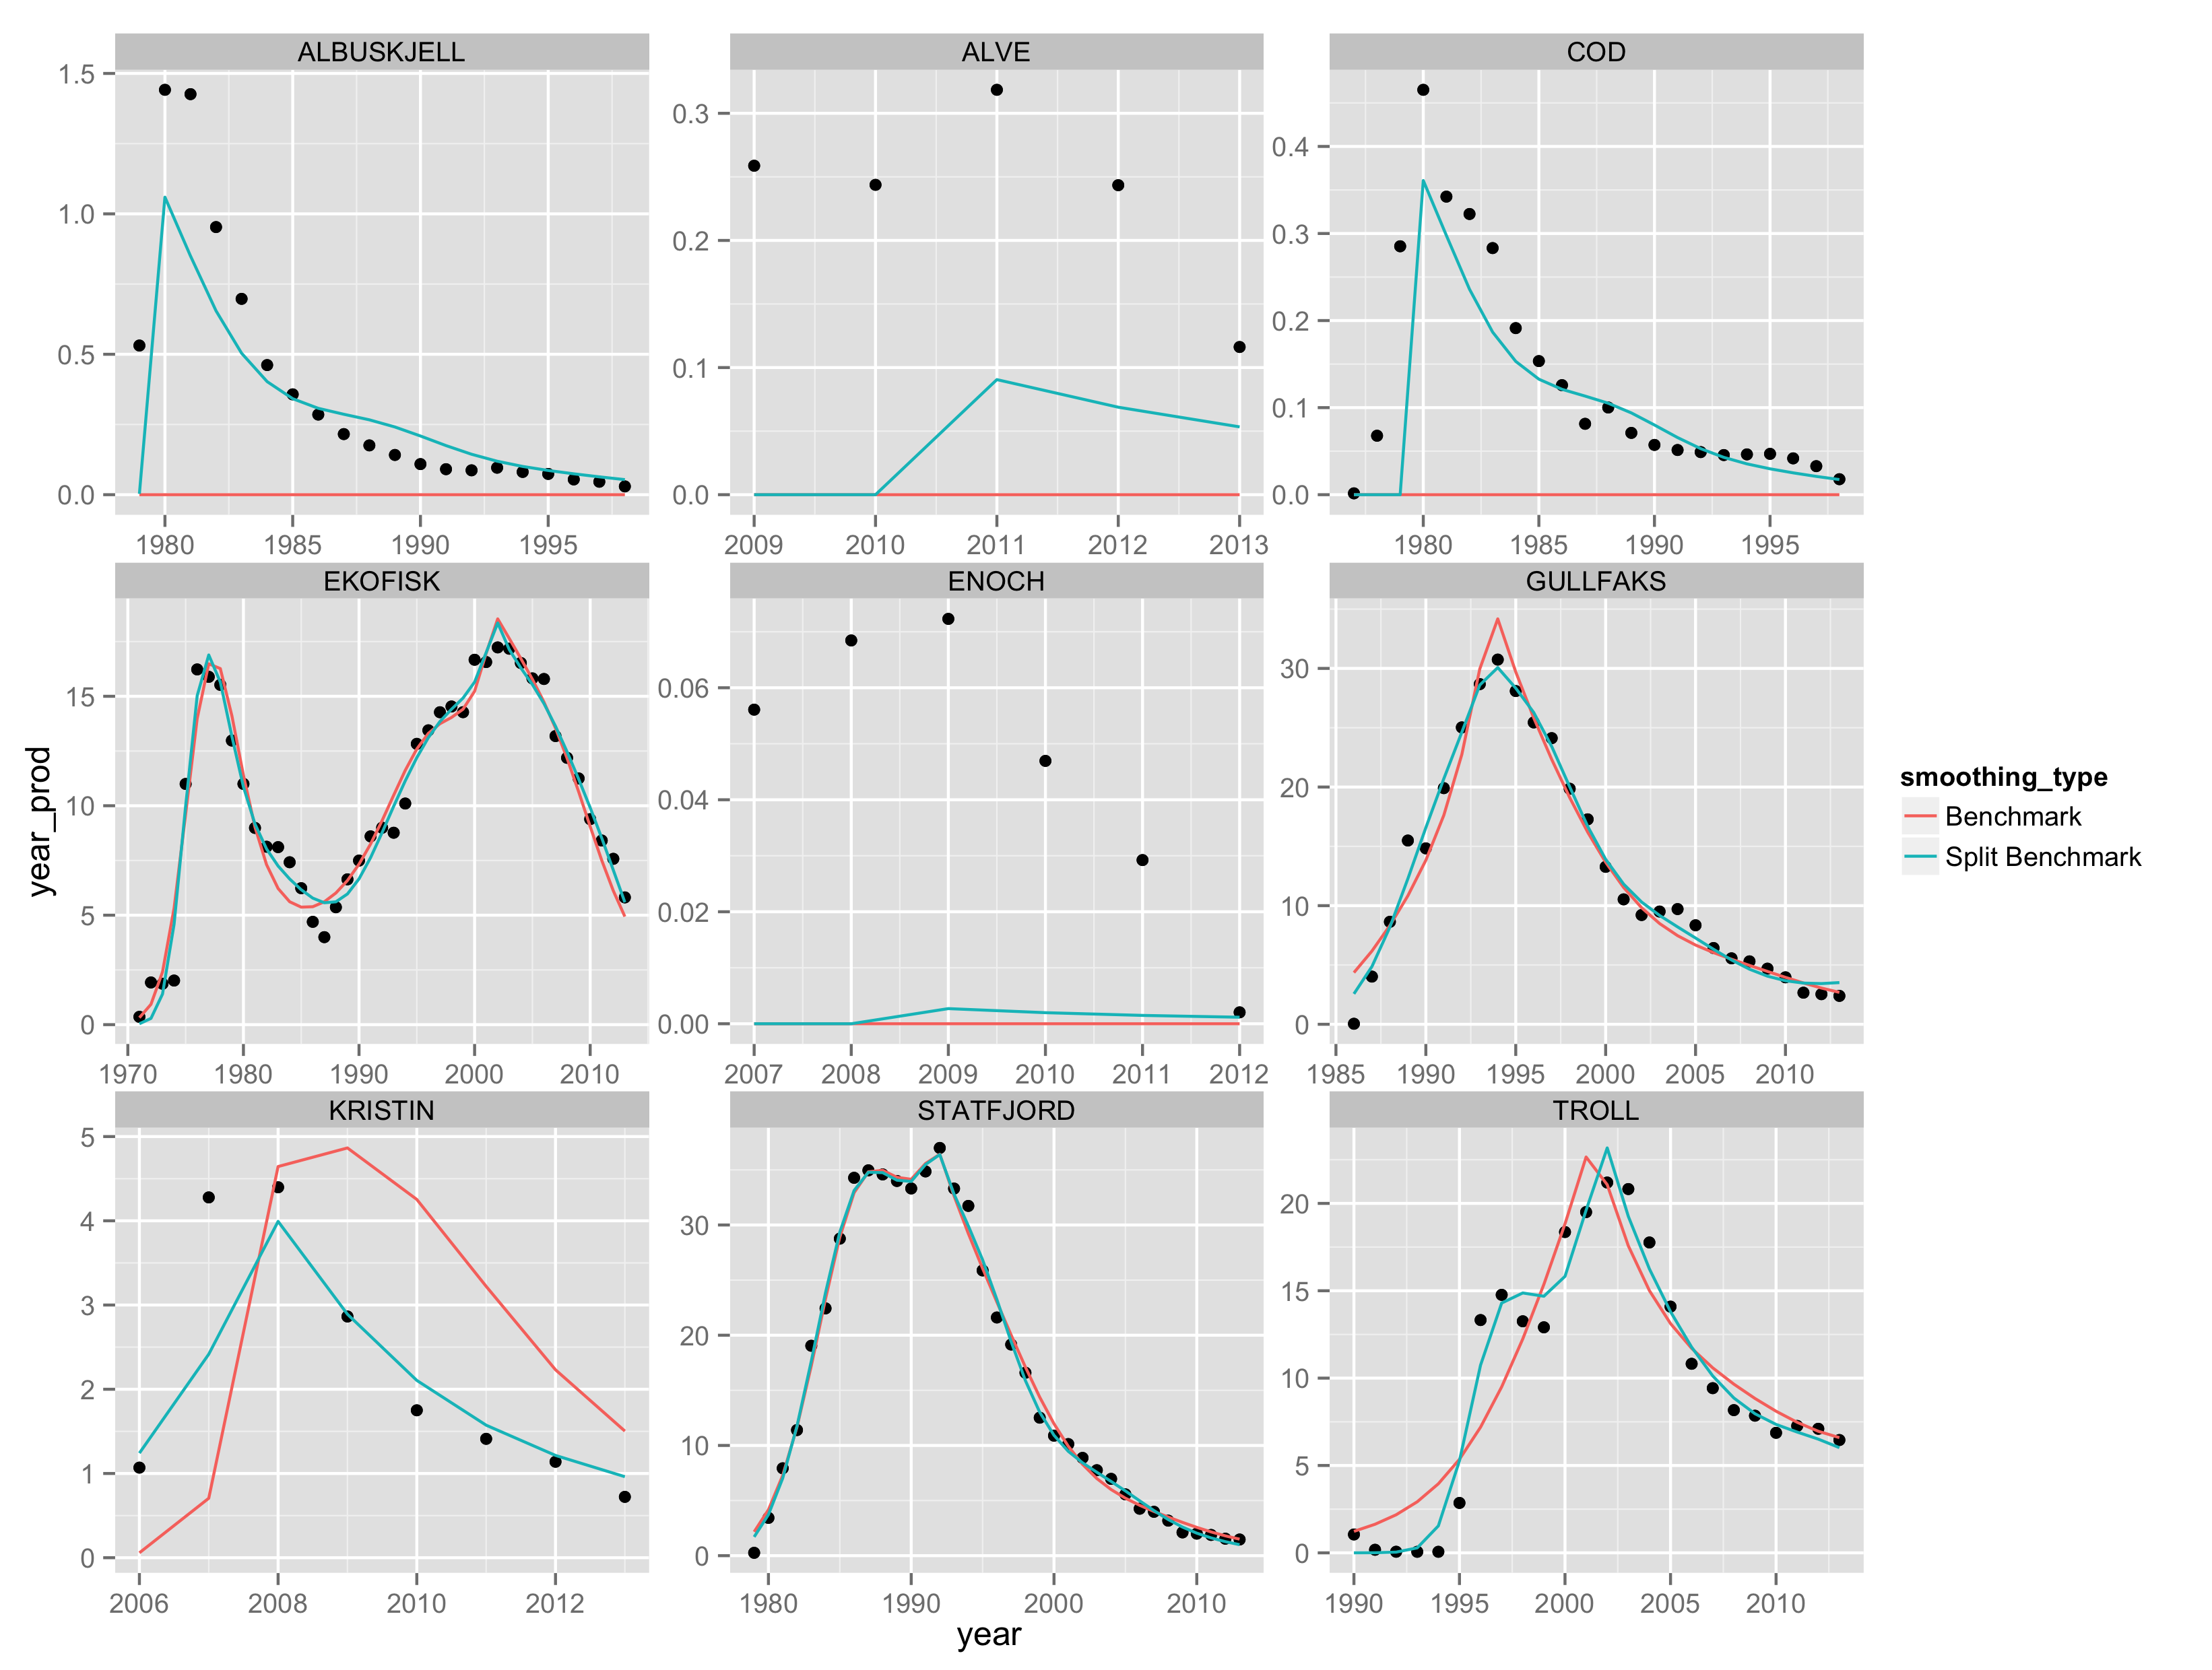
\includegraphics[width=.8\textwidth]{figures/bench_vs_split.png}
		
		\label{bench_vs_split}
	\end{figure}
\end{frame}


\begin{frame}[plain]
	\begin{figure}
		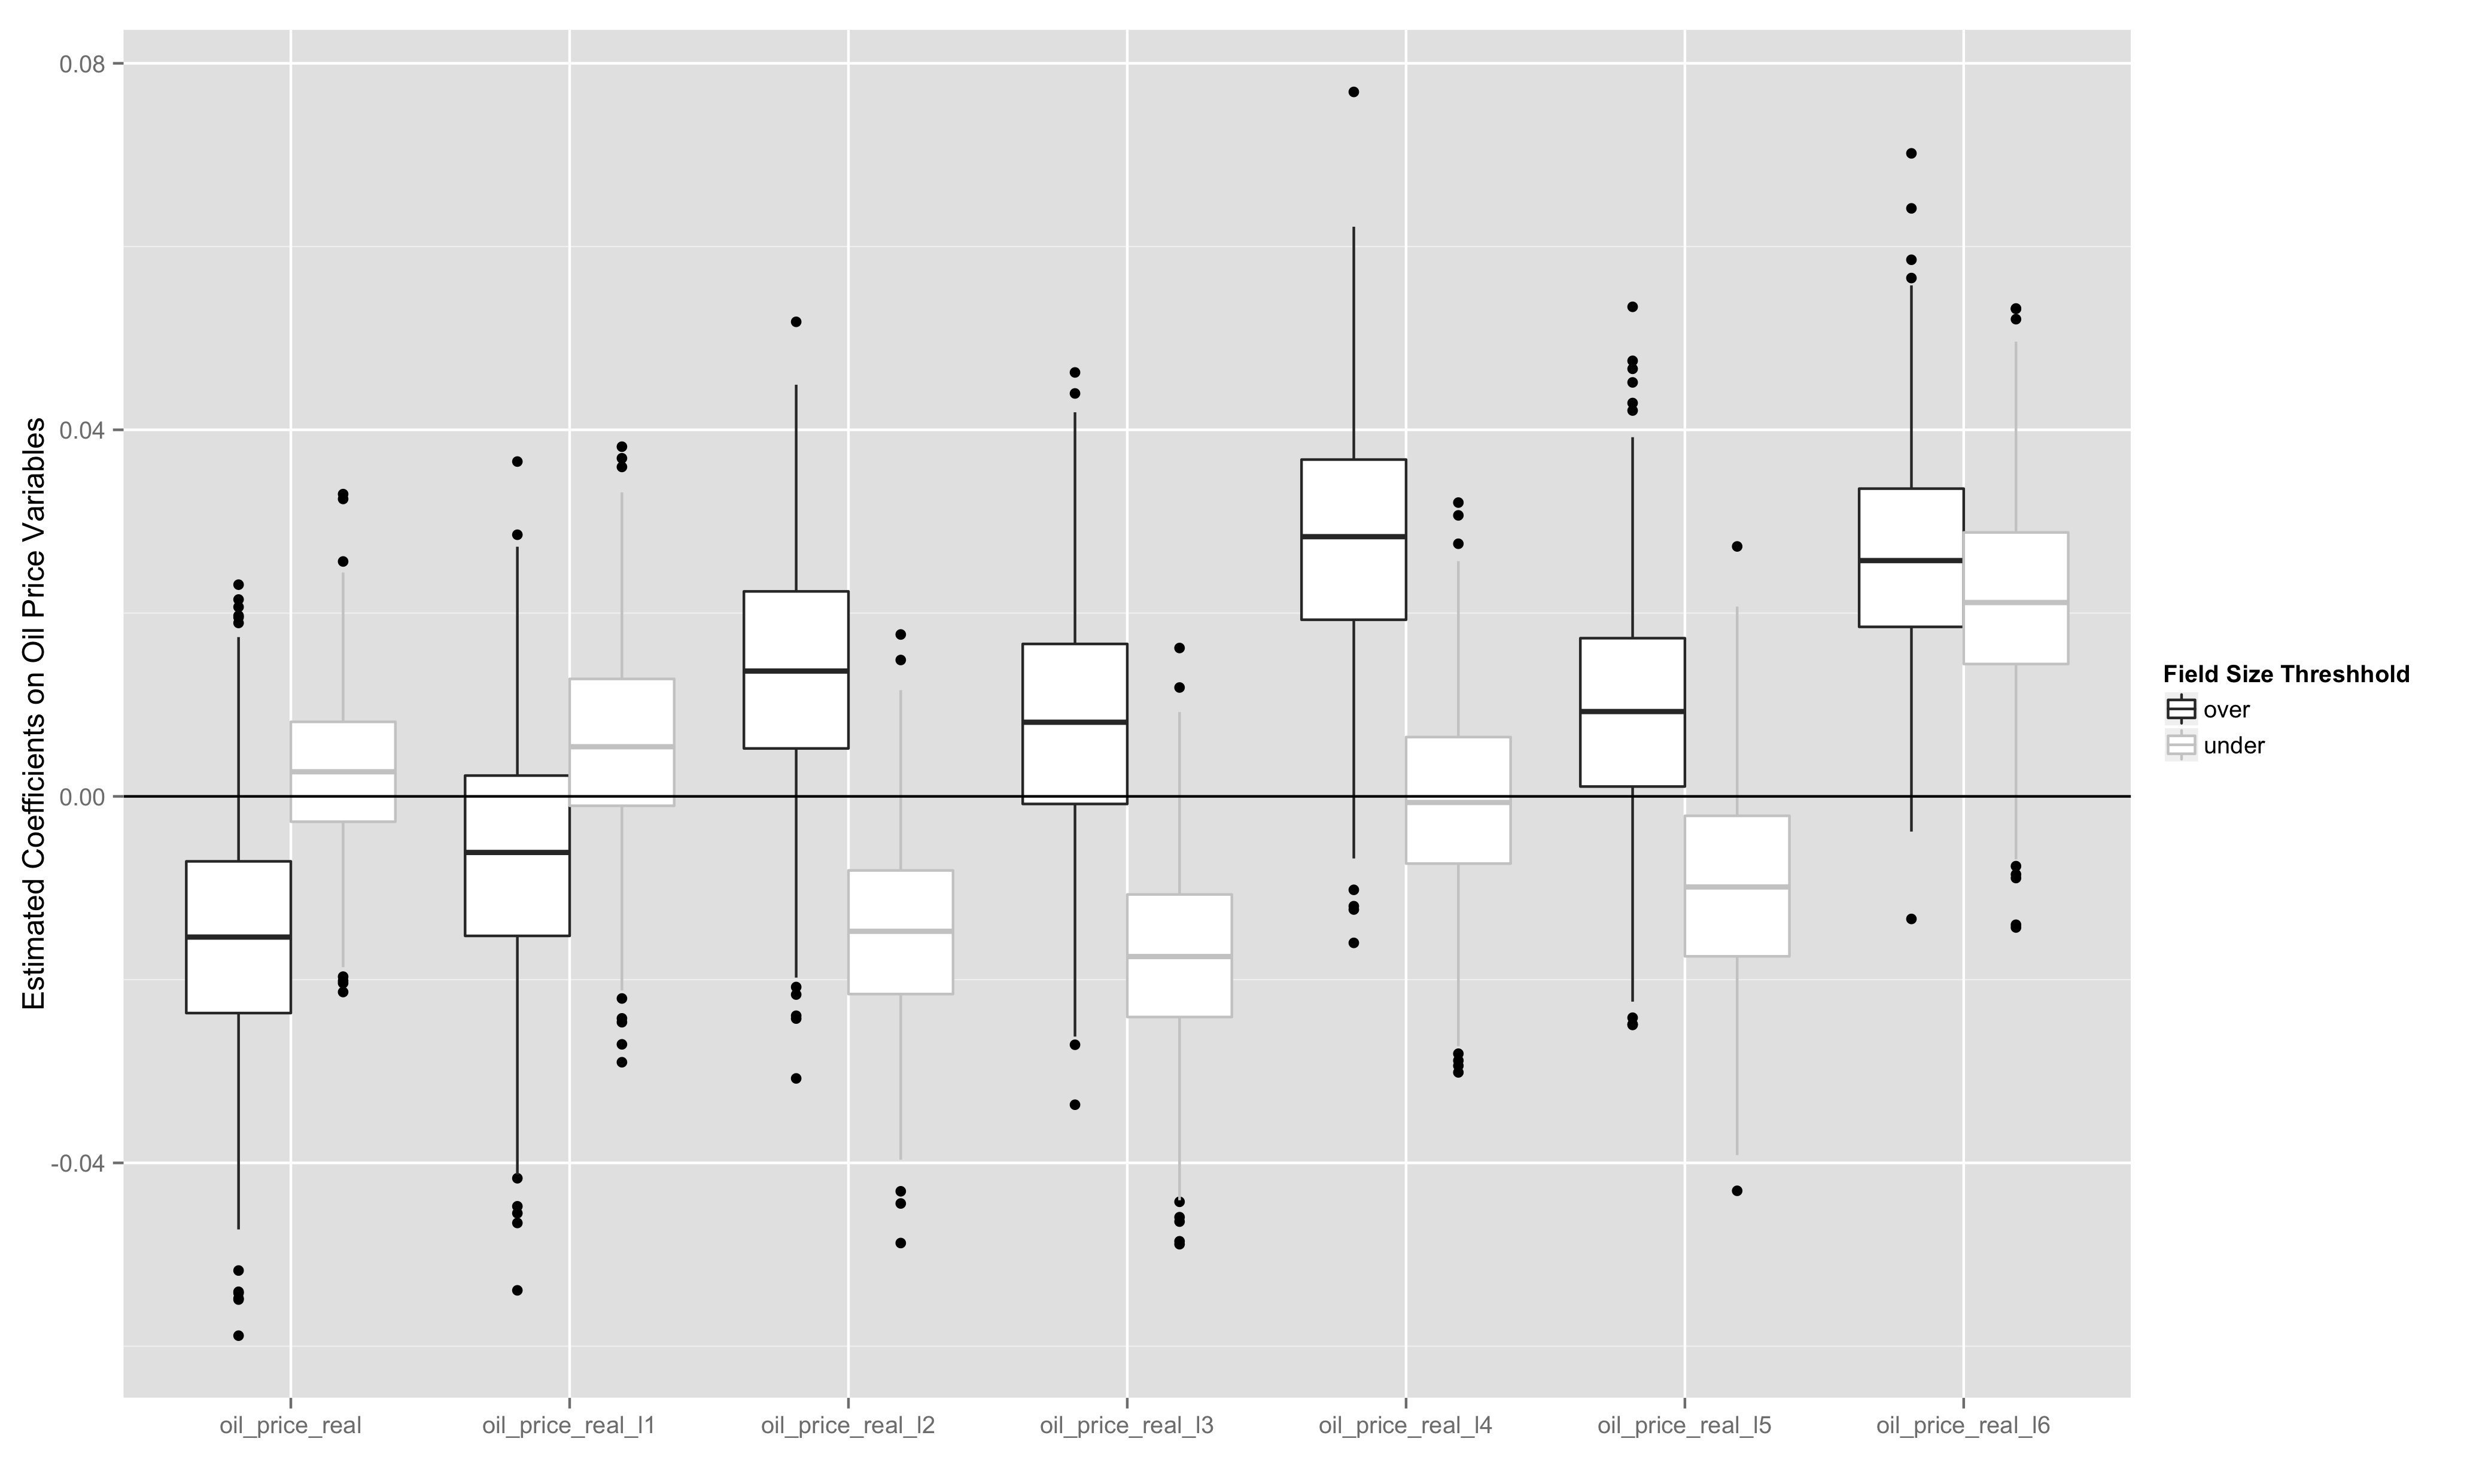
\includegraphics[width=.8\textwidth]{figures/gam_price_6_print.png}
		
		\label{gam_price_dirty_box}
	\end{figure}
\end{frame}

\begin{frame}[plain]
	\begin{figure}
	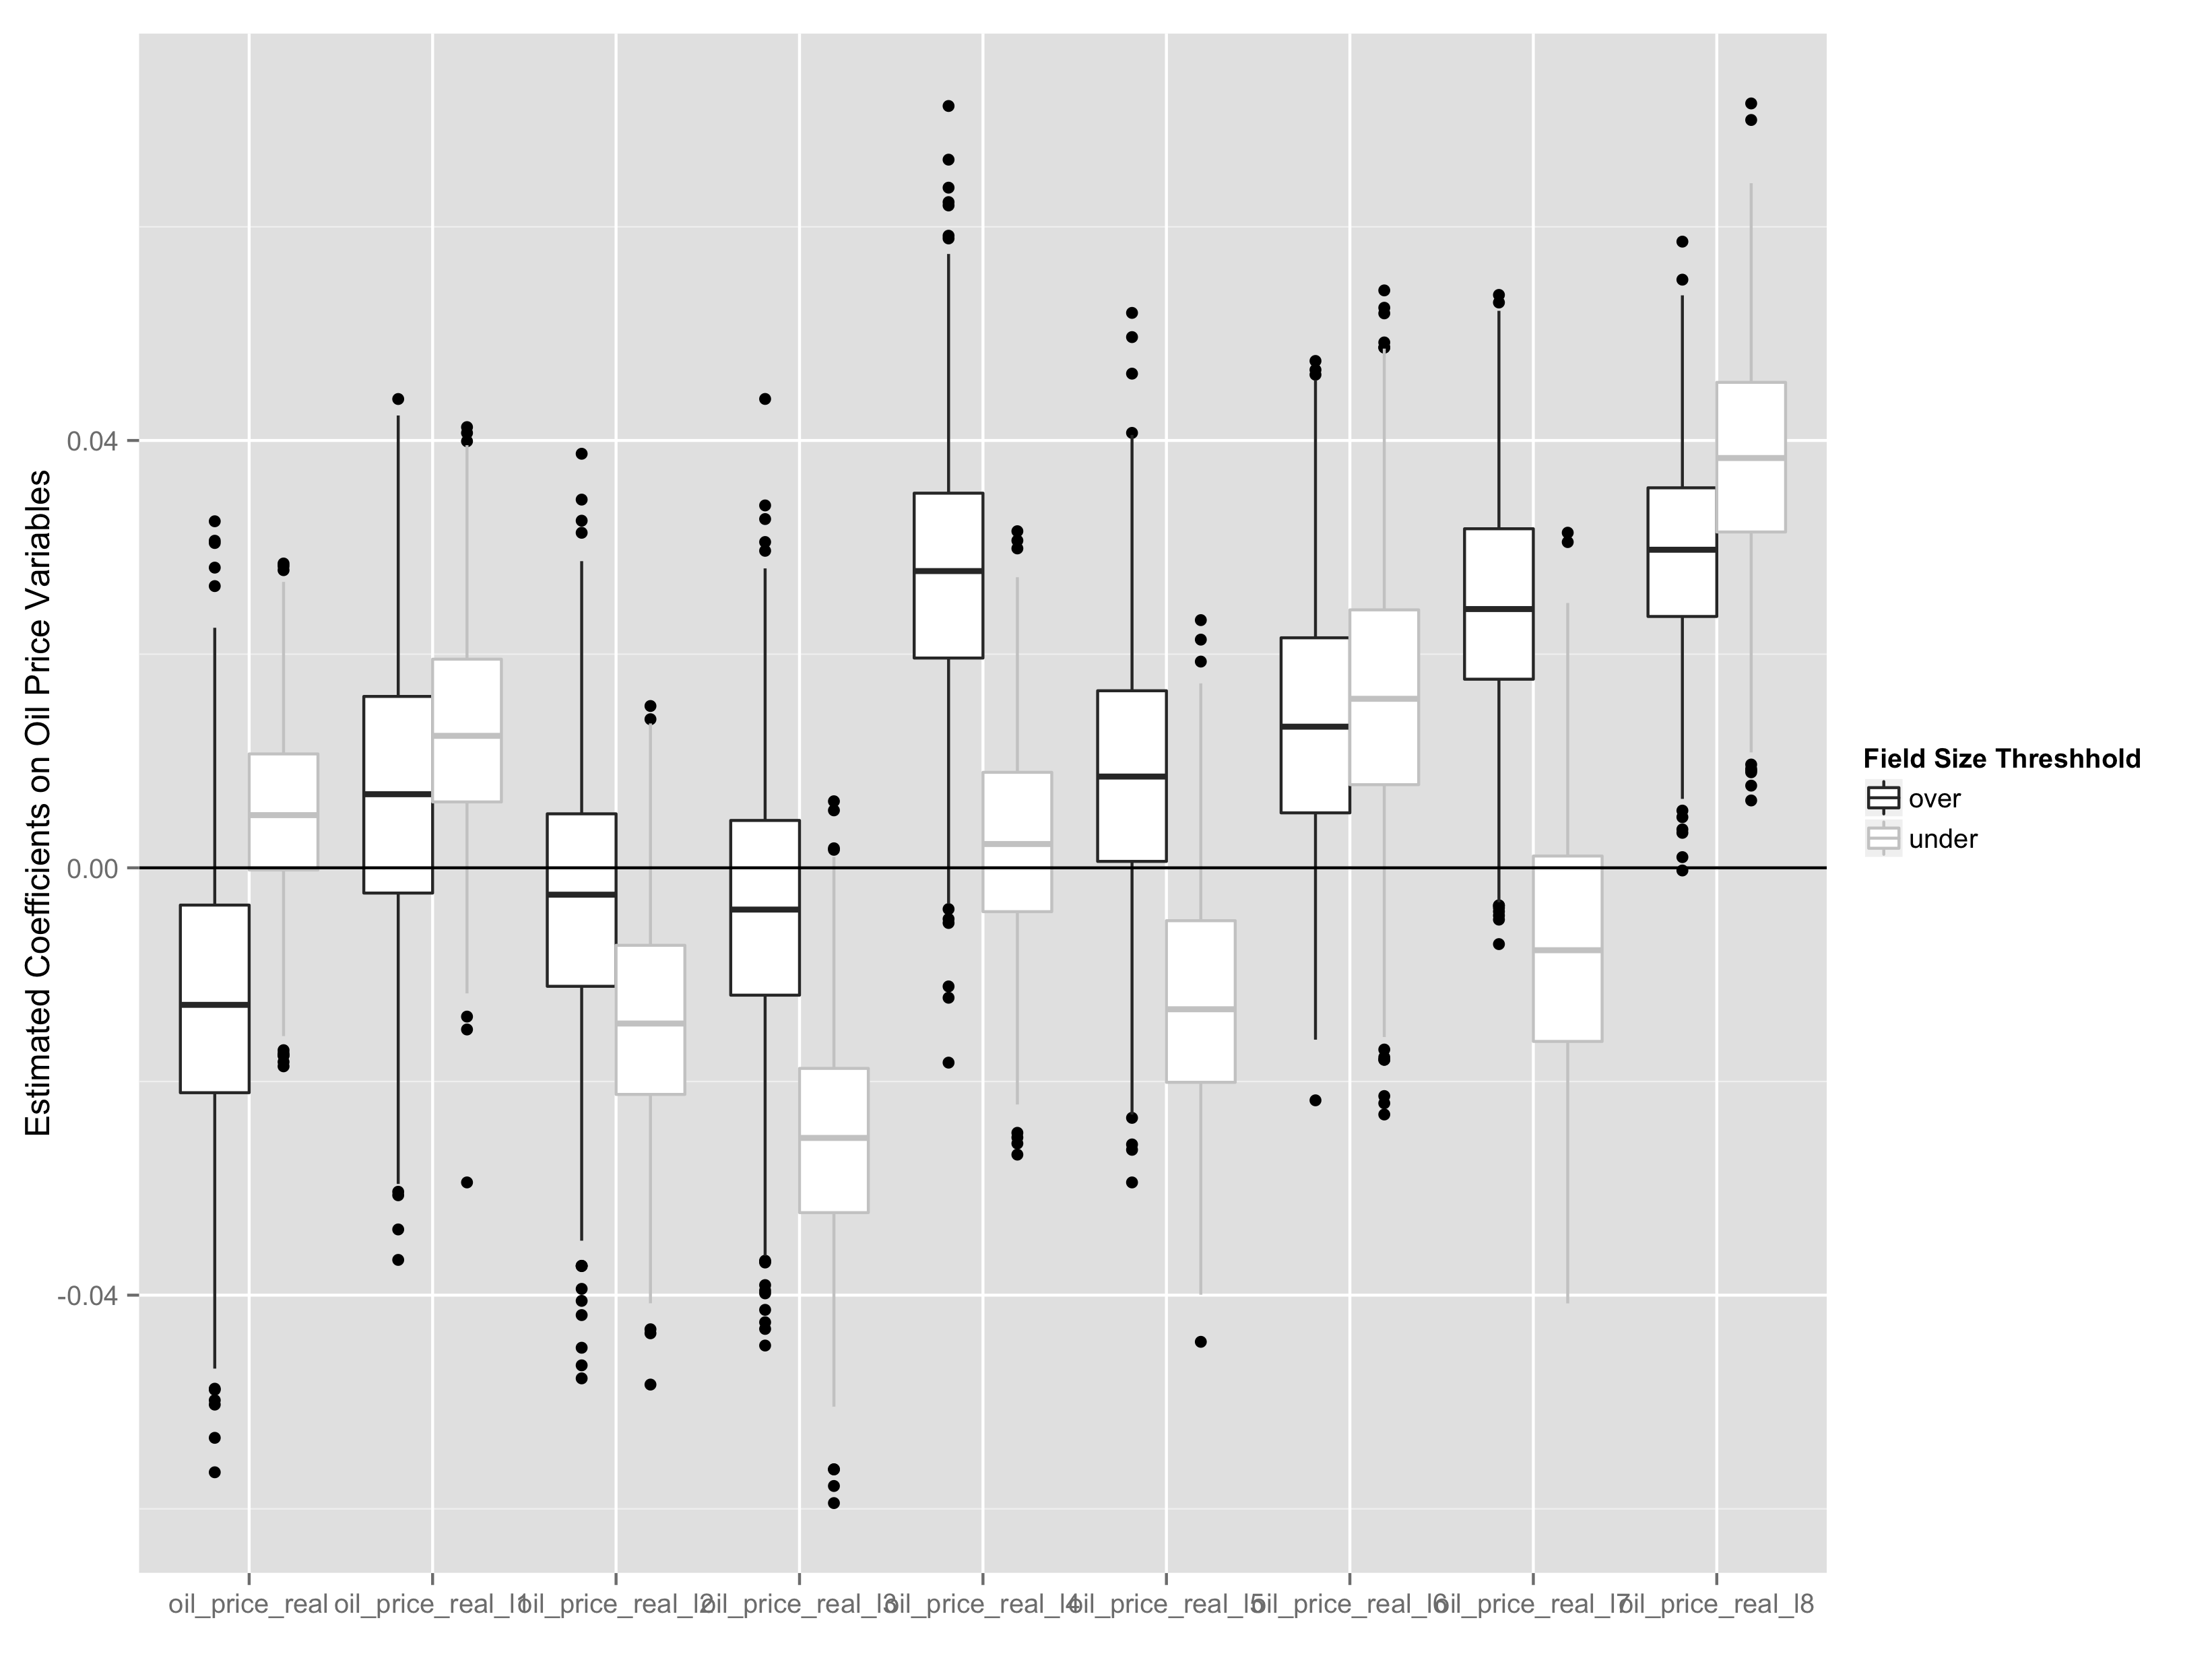
\includegraphics[width=.8\textwidth]{figures/gam_price_8_pres.png}
	% \caption{The coefficient estimates on the price terms where two additional lags are added to the model.  Significant positive results are found on the 8th lag for both large and small fields, providing evidence for adaptive price expectations by producers.}
	\label{gam_price_8}
	\end{figure}
\end{frame}

\begin{frame}[plain]
	\begin{figure}
	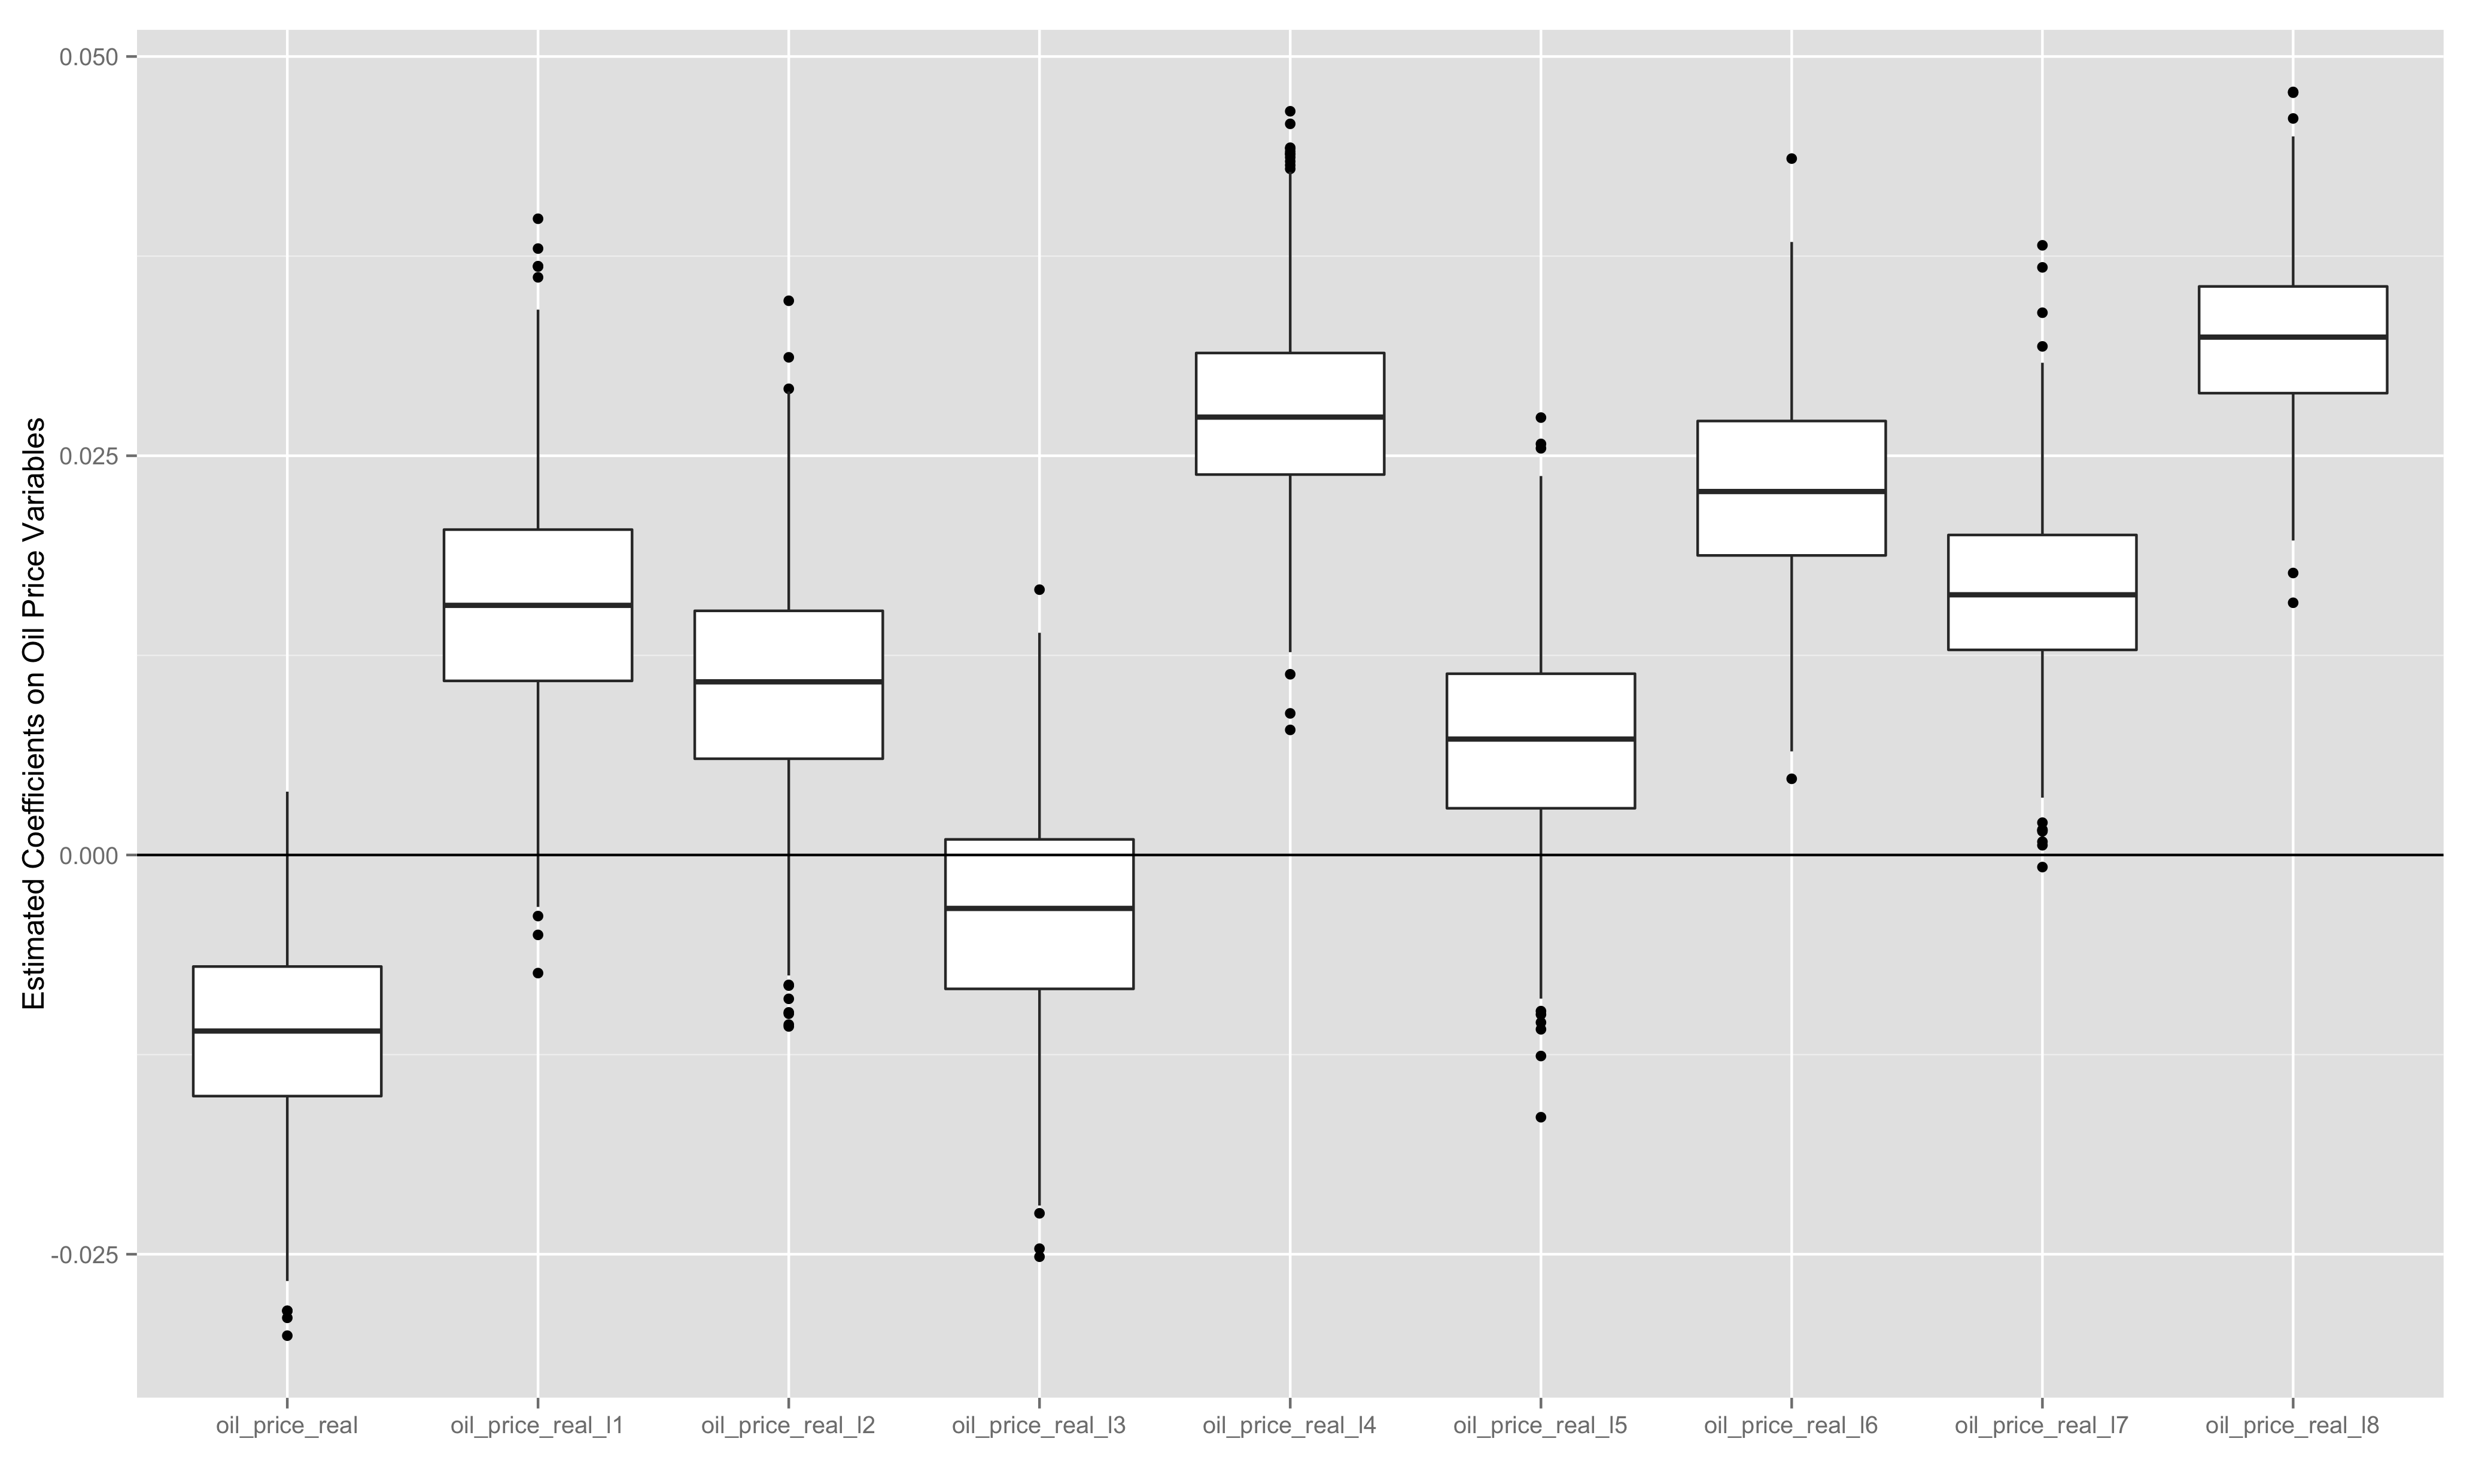
\includegraphics[width=1\textwidth]{figures/gam_price_pooled_print.png}
	\label{gam_price_pooled}
	\end{figure}
\end{frame}

\begin{frame}[plain]
	\begin{equation}
	\begin{split}
		Log(Investment_{i,t})&=f(time\_to\_peak_{i,t}, total\_recoverable\_oil_i) \\
		& \quad + f(peak\_to\_end_{i,t}, total\_recoverable\_oil_i) \\
		& \quad + \alpha oil_production_{i,t} \\
		& \quad + \beta_1 oil\_price + \beta_2 oil\_price\_l1 + ... +  \epsilon
	\end{split}
	\label{gam_invest_eqn}
	\end{equation}
\end{frame}

\begin{frame}[plain]
\begin{figure}
	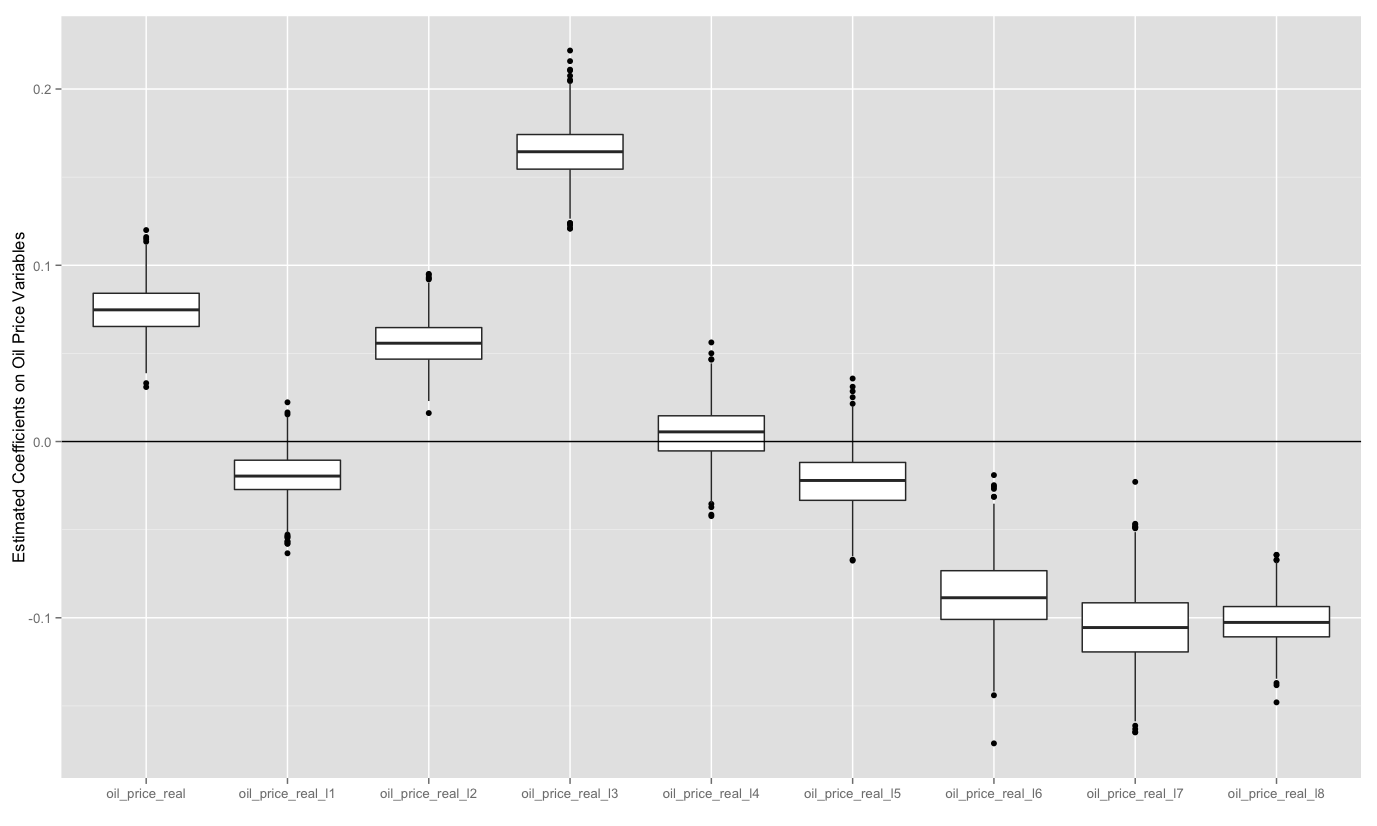
\includegraphics[width=1\textwidth]{figures/invest_pooled_print.png}
	\label{gam_price_invest_box}
\end{figure}
\end{frame}


\begin{frame}[plain]
	\begin{figure}
	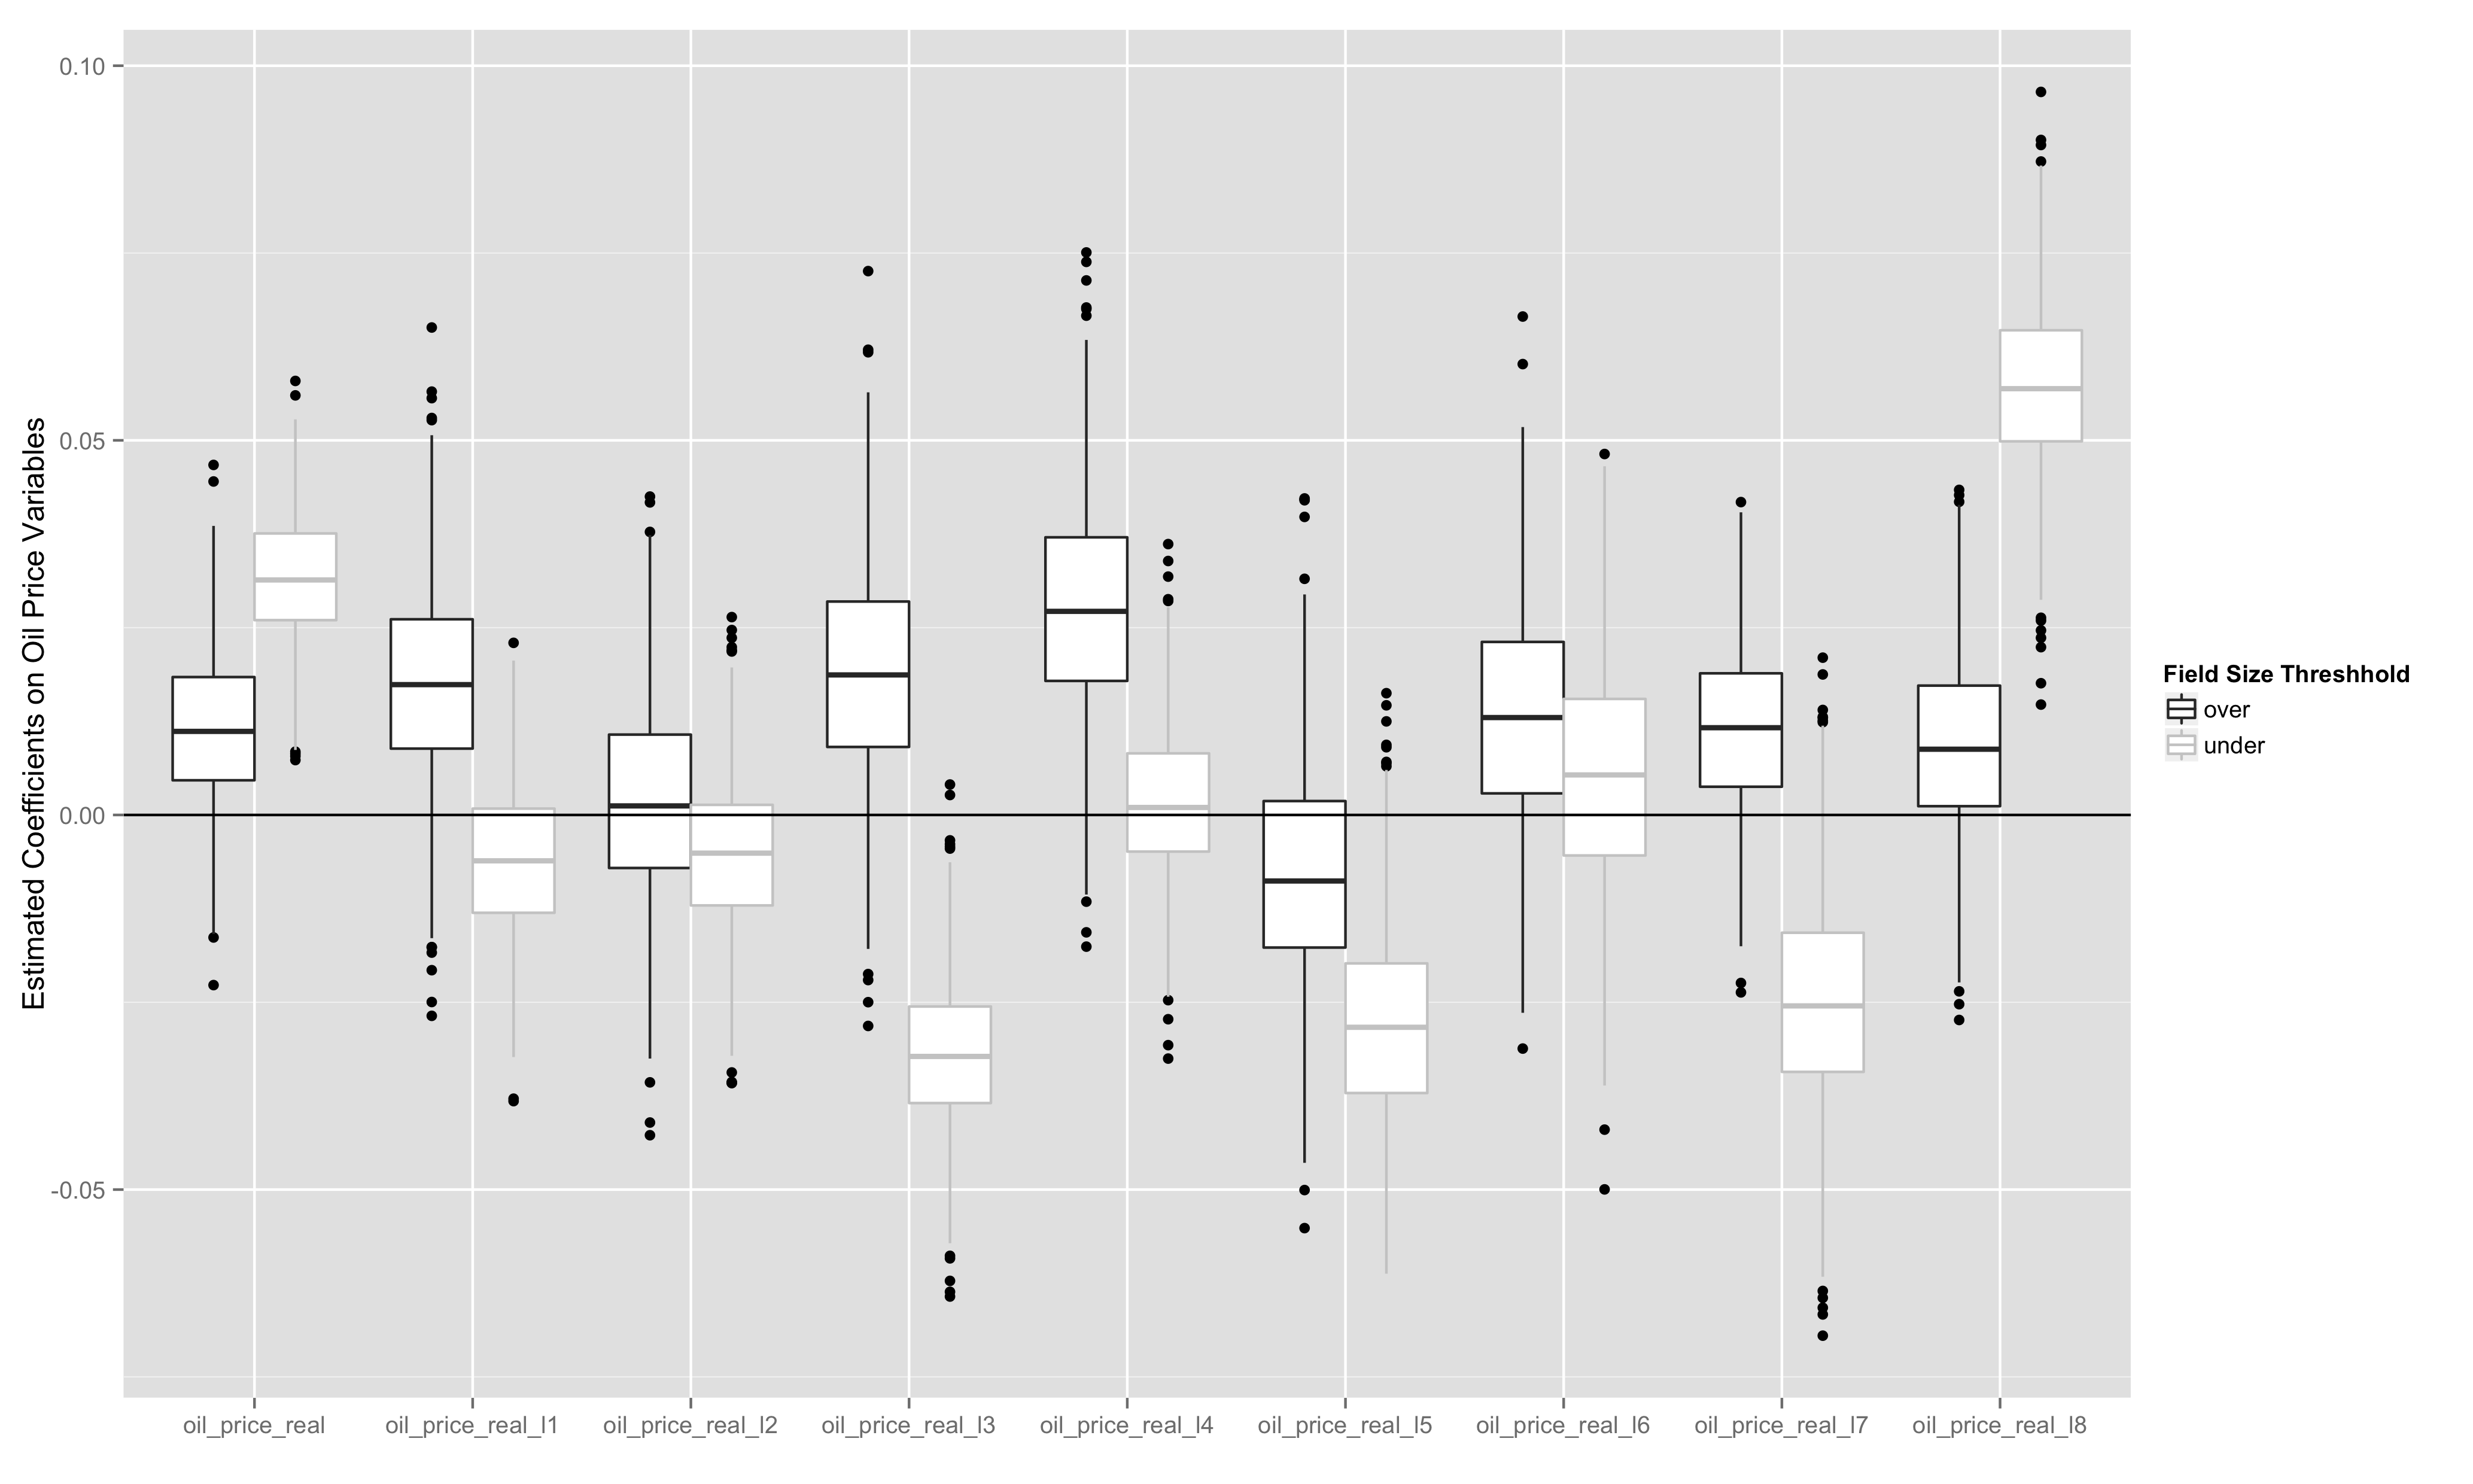
\includegraphics[width=1\textwidth]{figures/gam_postpeak_print.png}
	% \caption{The estimated coefficients on the price terms in a model of oil field production in depleting fields.  No significant coefficients are estimated except for on the 8th lag of small fields.  This effect is not, however, robust to changes in specification.}
	\label{gam_postpeak_pres}
	\end{figure}
\end{frame}


\begin{frame}[plain]
	\begin{figure}
	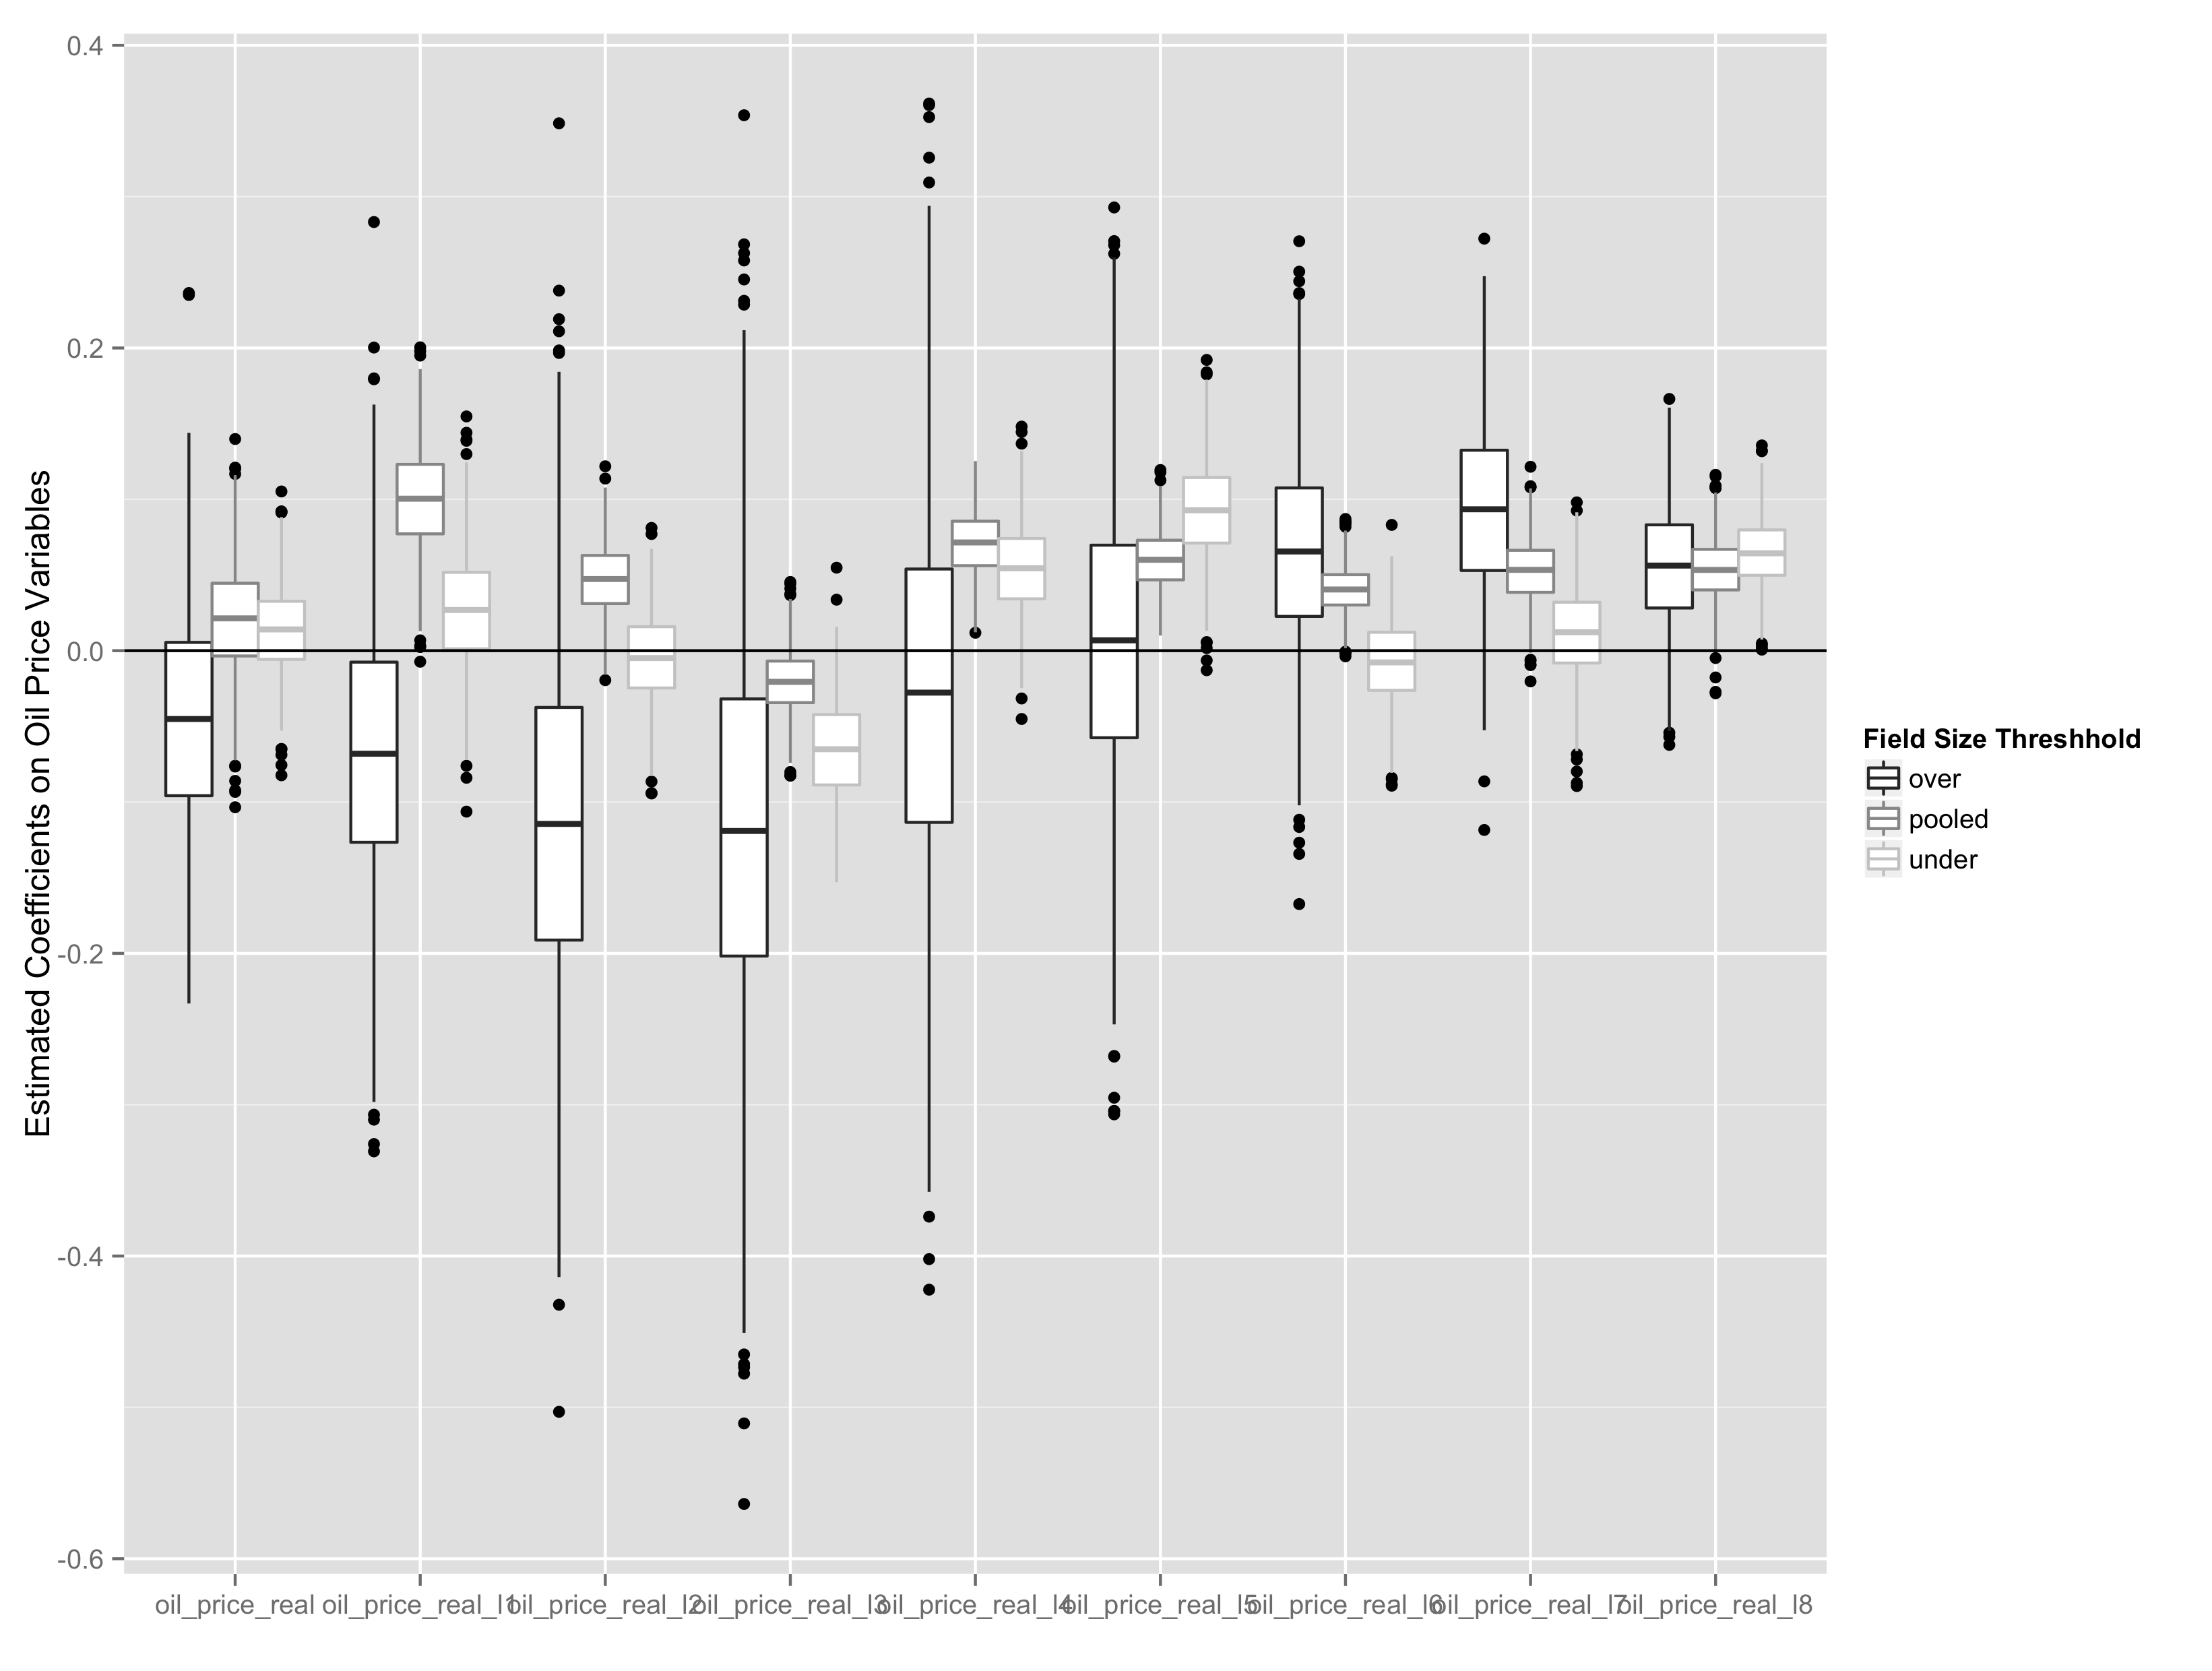
\includegraphics[width=1\textwidth]{figures/gam_prepeak_pres.png}
	% \caption{The estimated coefficients on the price terms in a model of fields in the build-out phase.  For large fields, positive coefficients are estimated at the 6th, 7th and 8th lag, but the estimates are imprecise and not statistically significant.  Significant positive coefficients are estimated for small fields at the fifth and eighth lag.  In a pooled model, significant positive coefficients are found at the fourth through eight lags.}
	\label{gam_prepeak_print}
	\end{figure}
\end{frame}

\begin{frame}[plain]
	\begin{figure}
		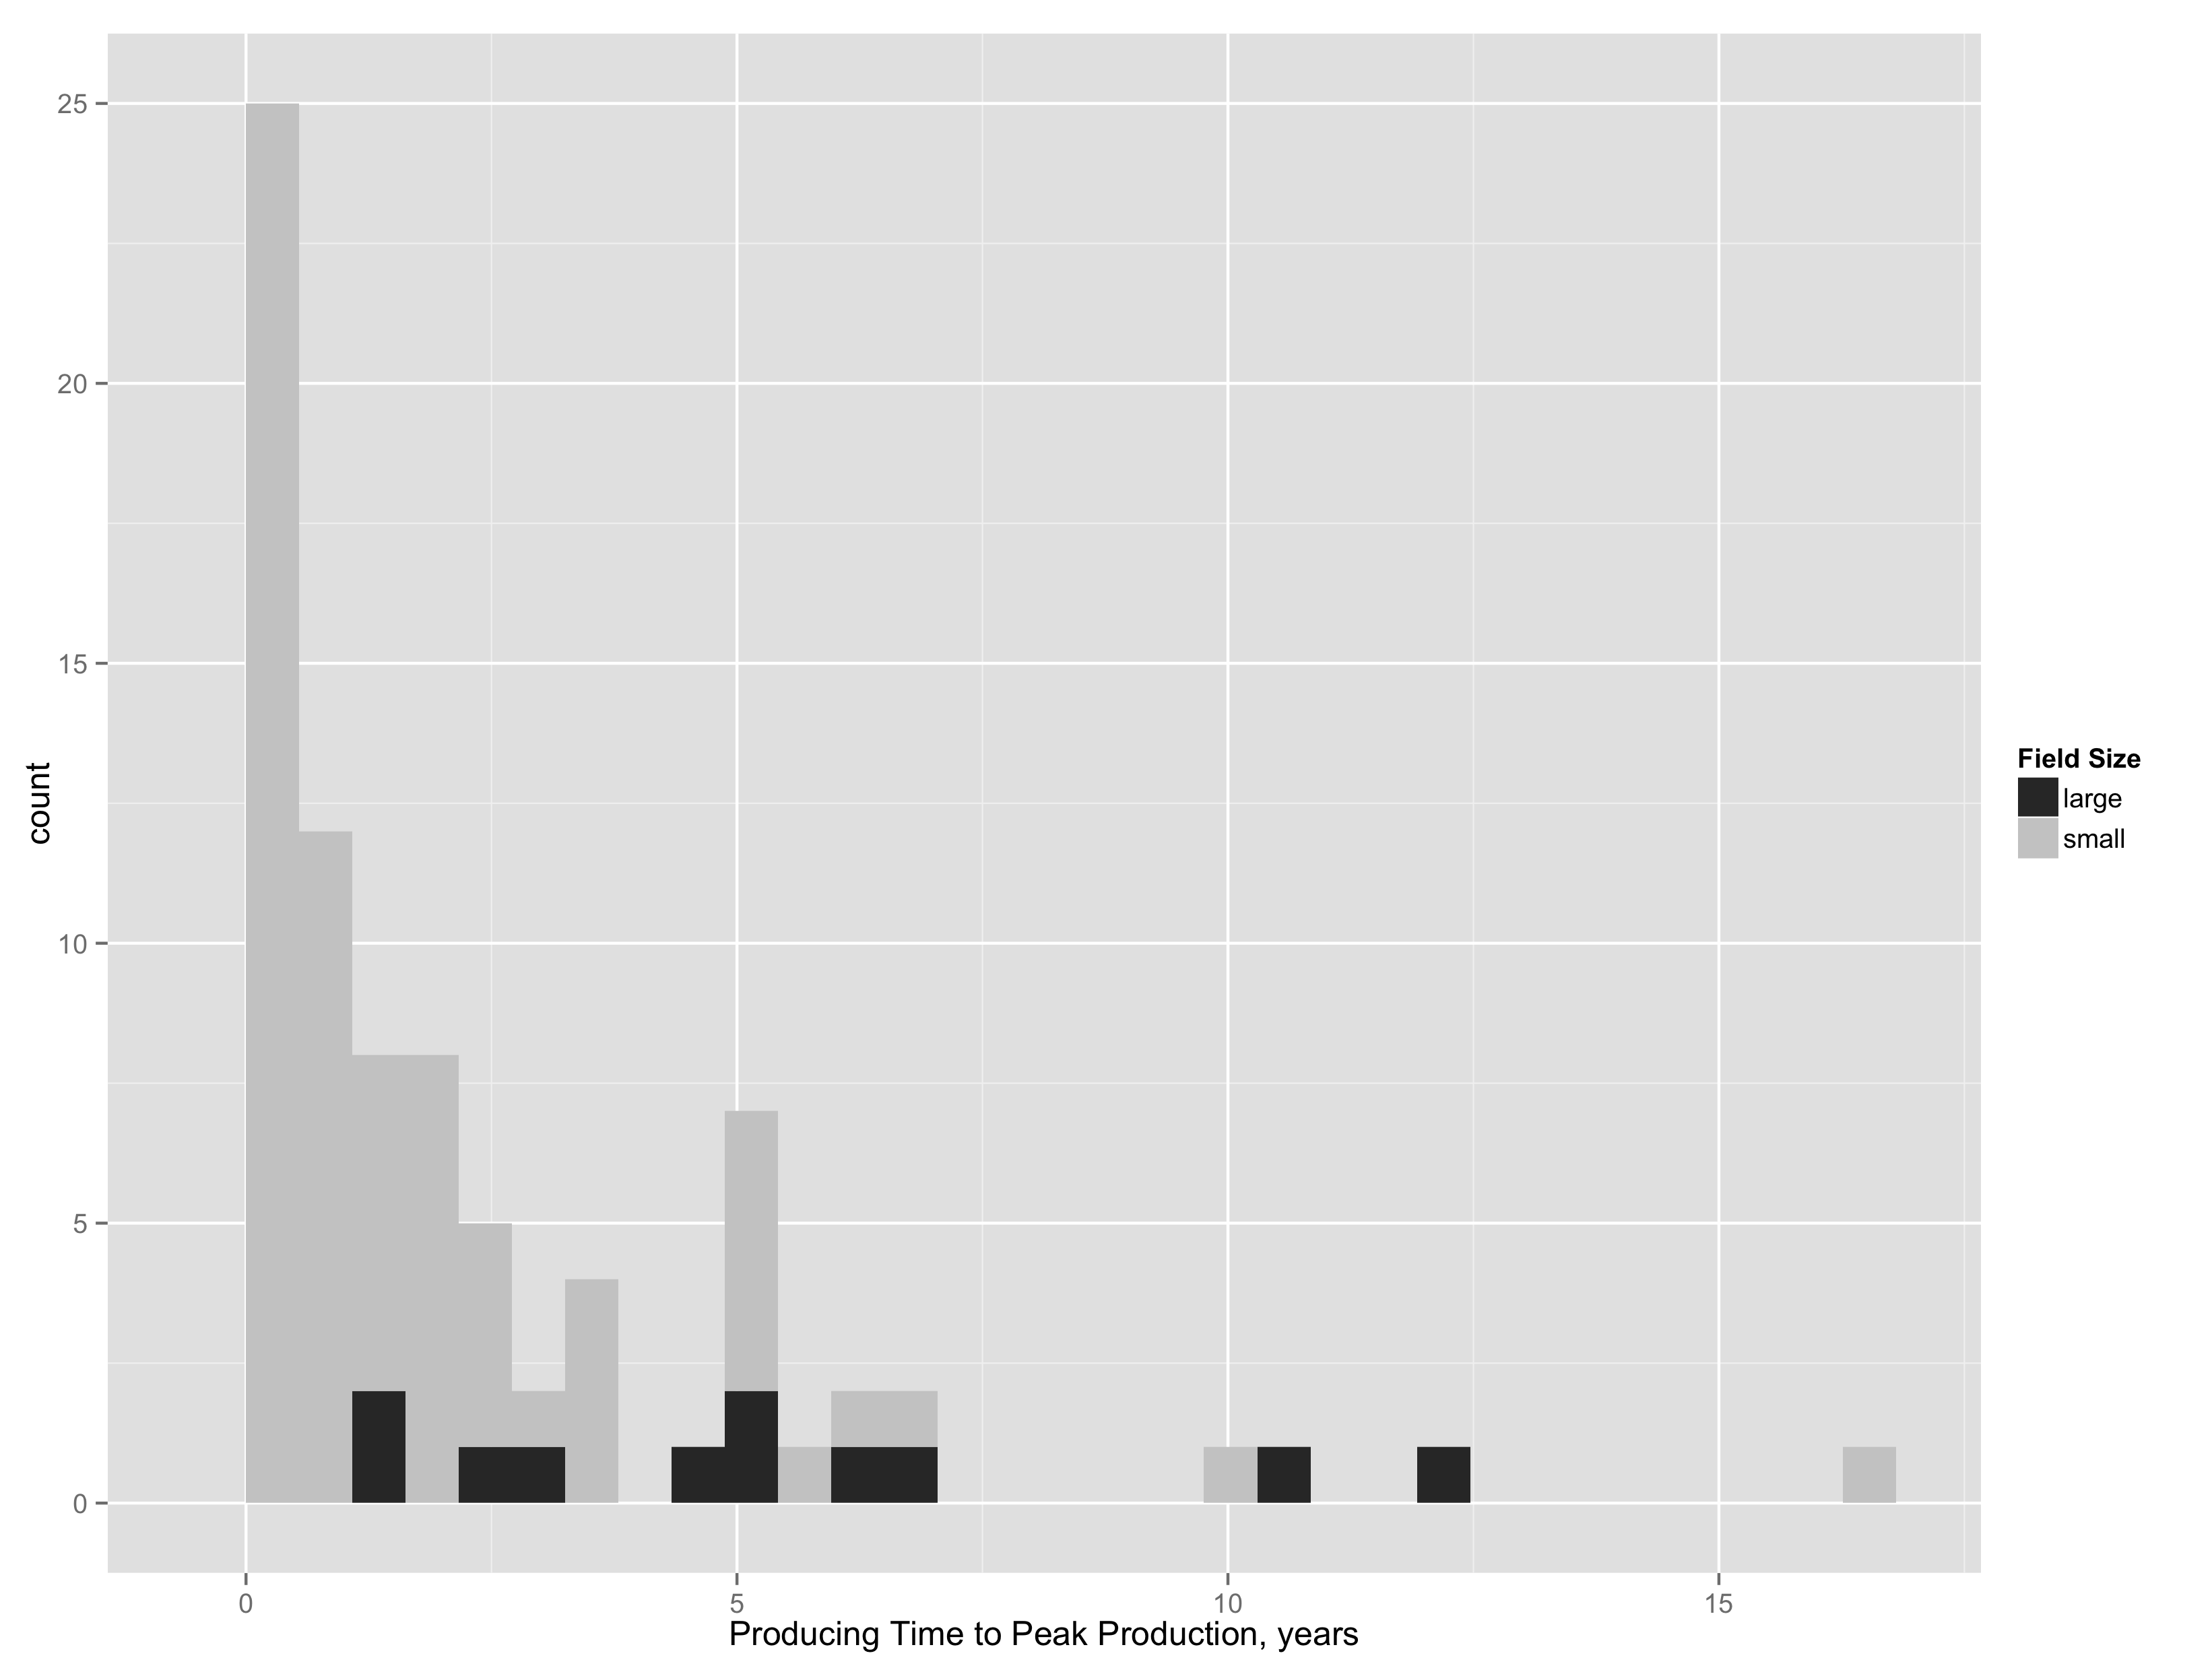
\includegraphics[width=.8\textwidth]{figures/field_time_to_peak_pres.png}		
		\label{field_time_to_peak}
	\end{figure}
\end{frame}


\begin{frame}[plain]
	\begin{figure}
		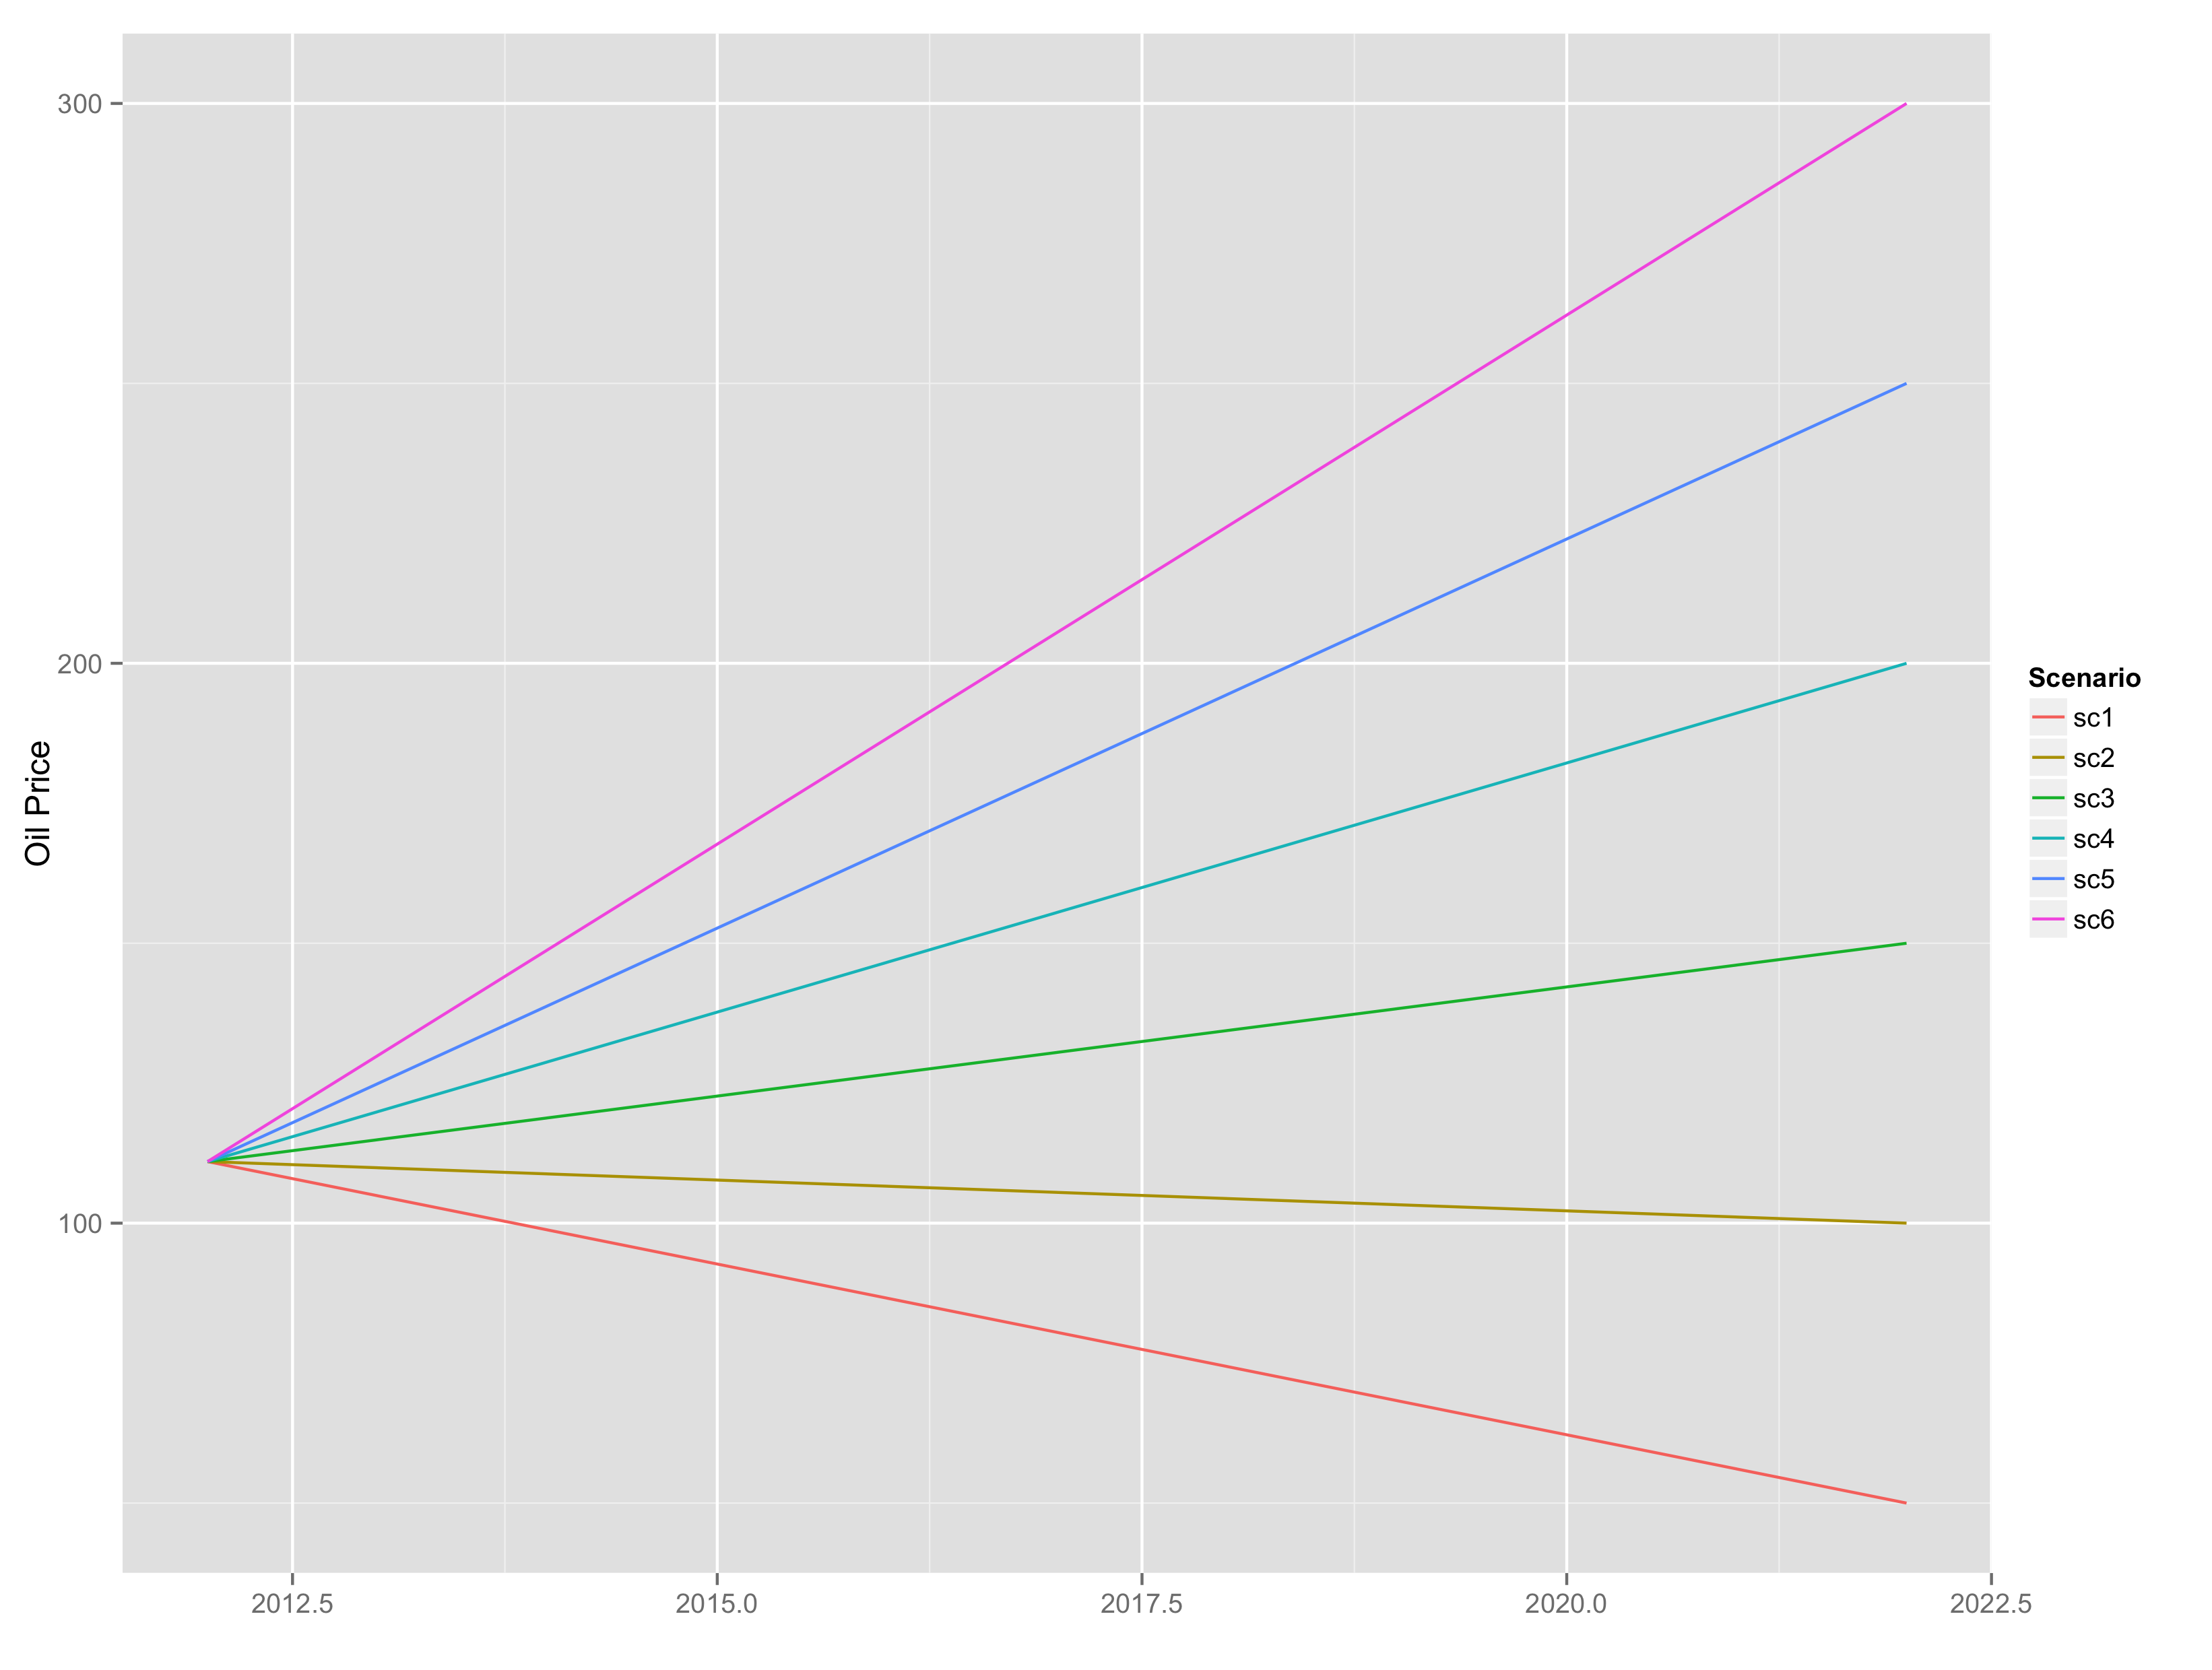
\includegraphics[width=.8\textwidth]{figures/price_scenario.png}
		
		\label{price_scenario}
	\end{figure}
\end{frame}

\begin{frame}[plain]
	\begin{figure}
		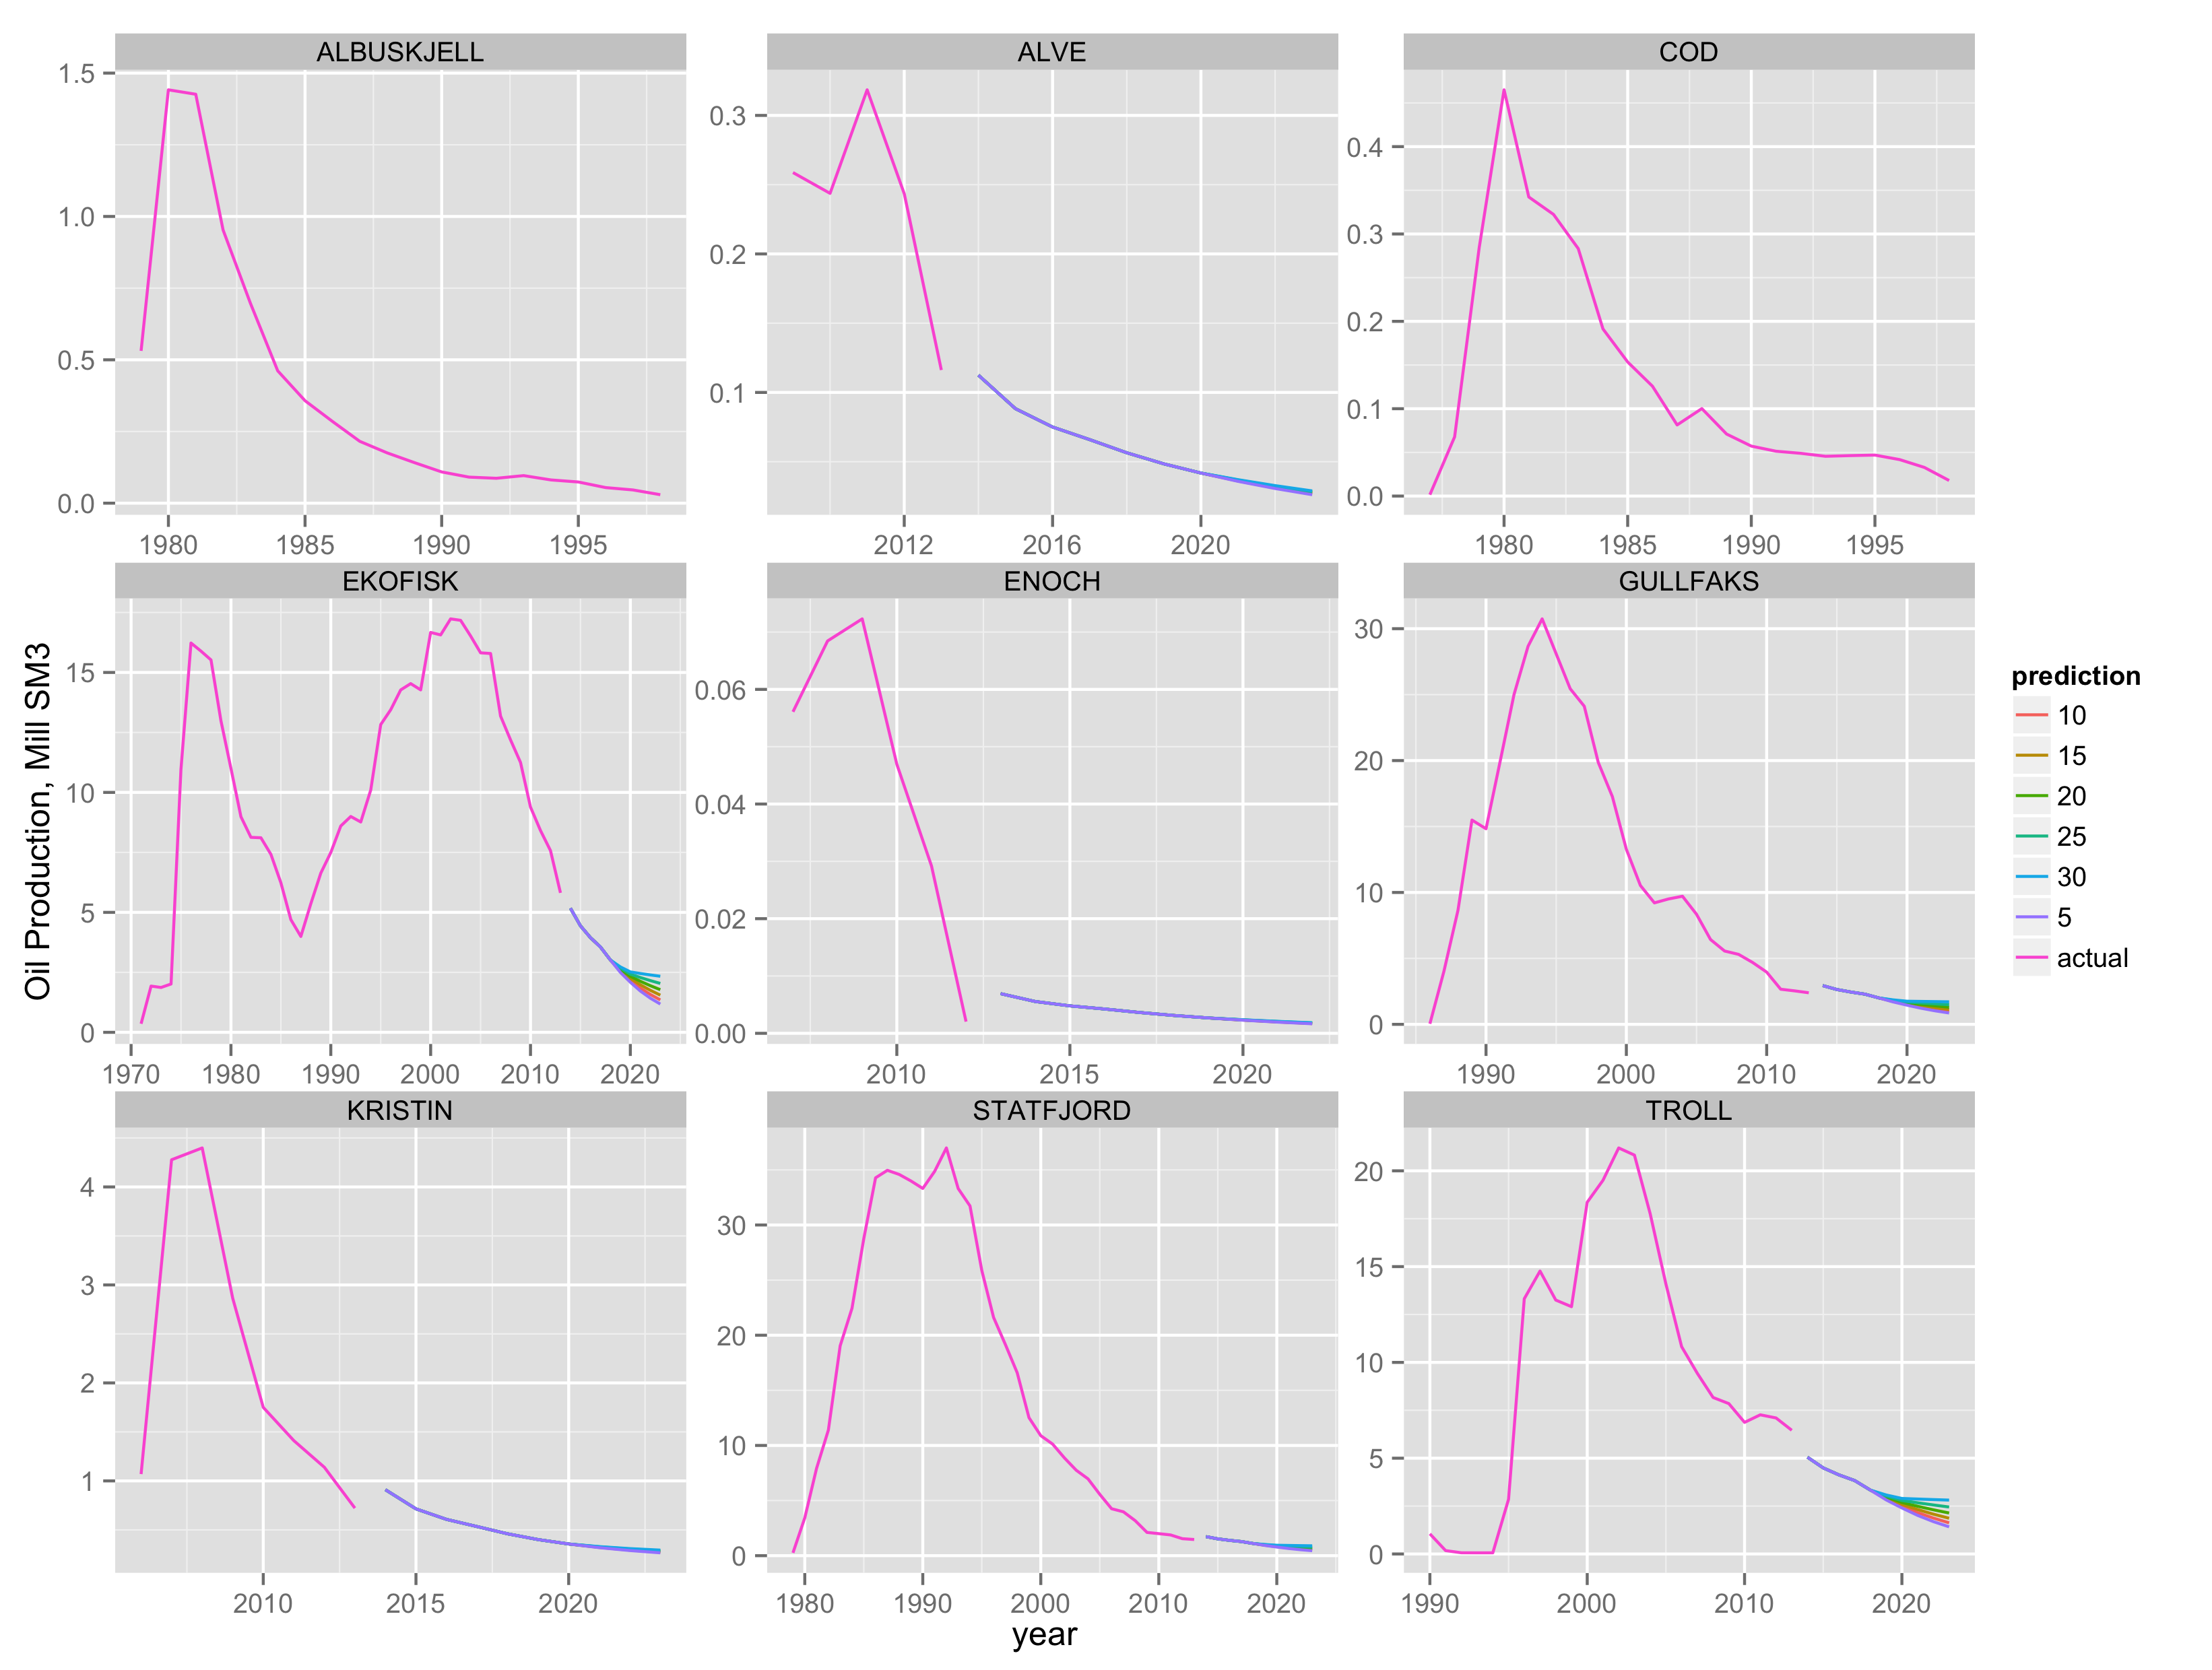
\includegraphics[width=.8\textwidth]{figures/field_lev_forecast.png}		
		\label{field_lev_forecast}
	\end{figure}

\end{frame}


\begin{frame}[plain]
	\begin{figure}
		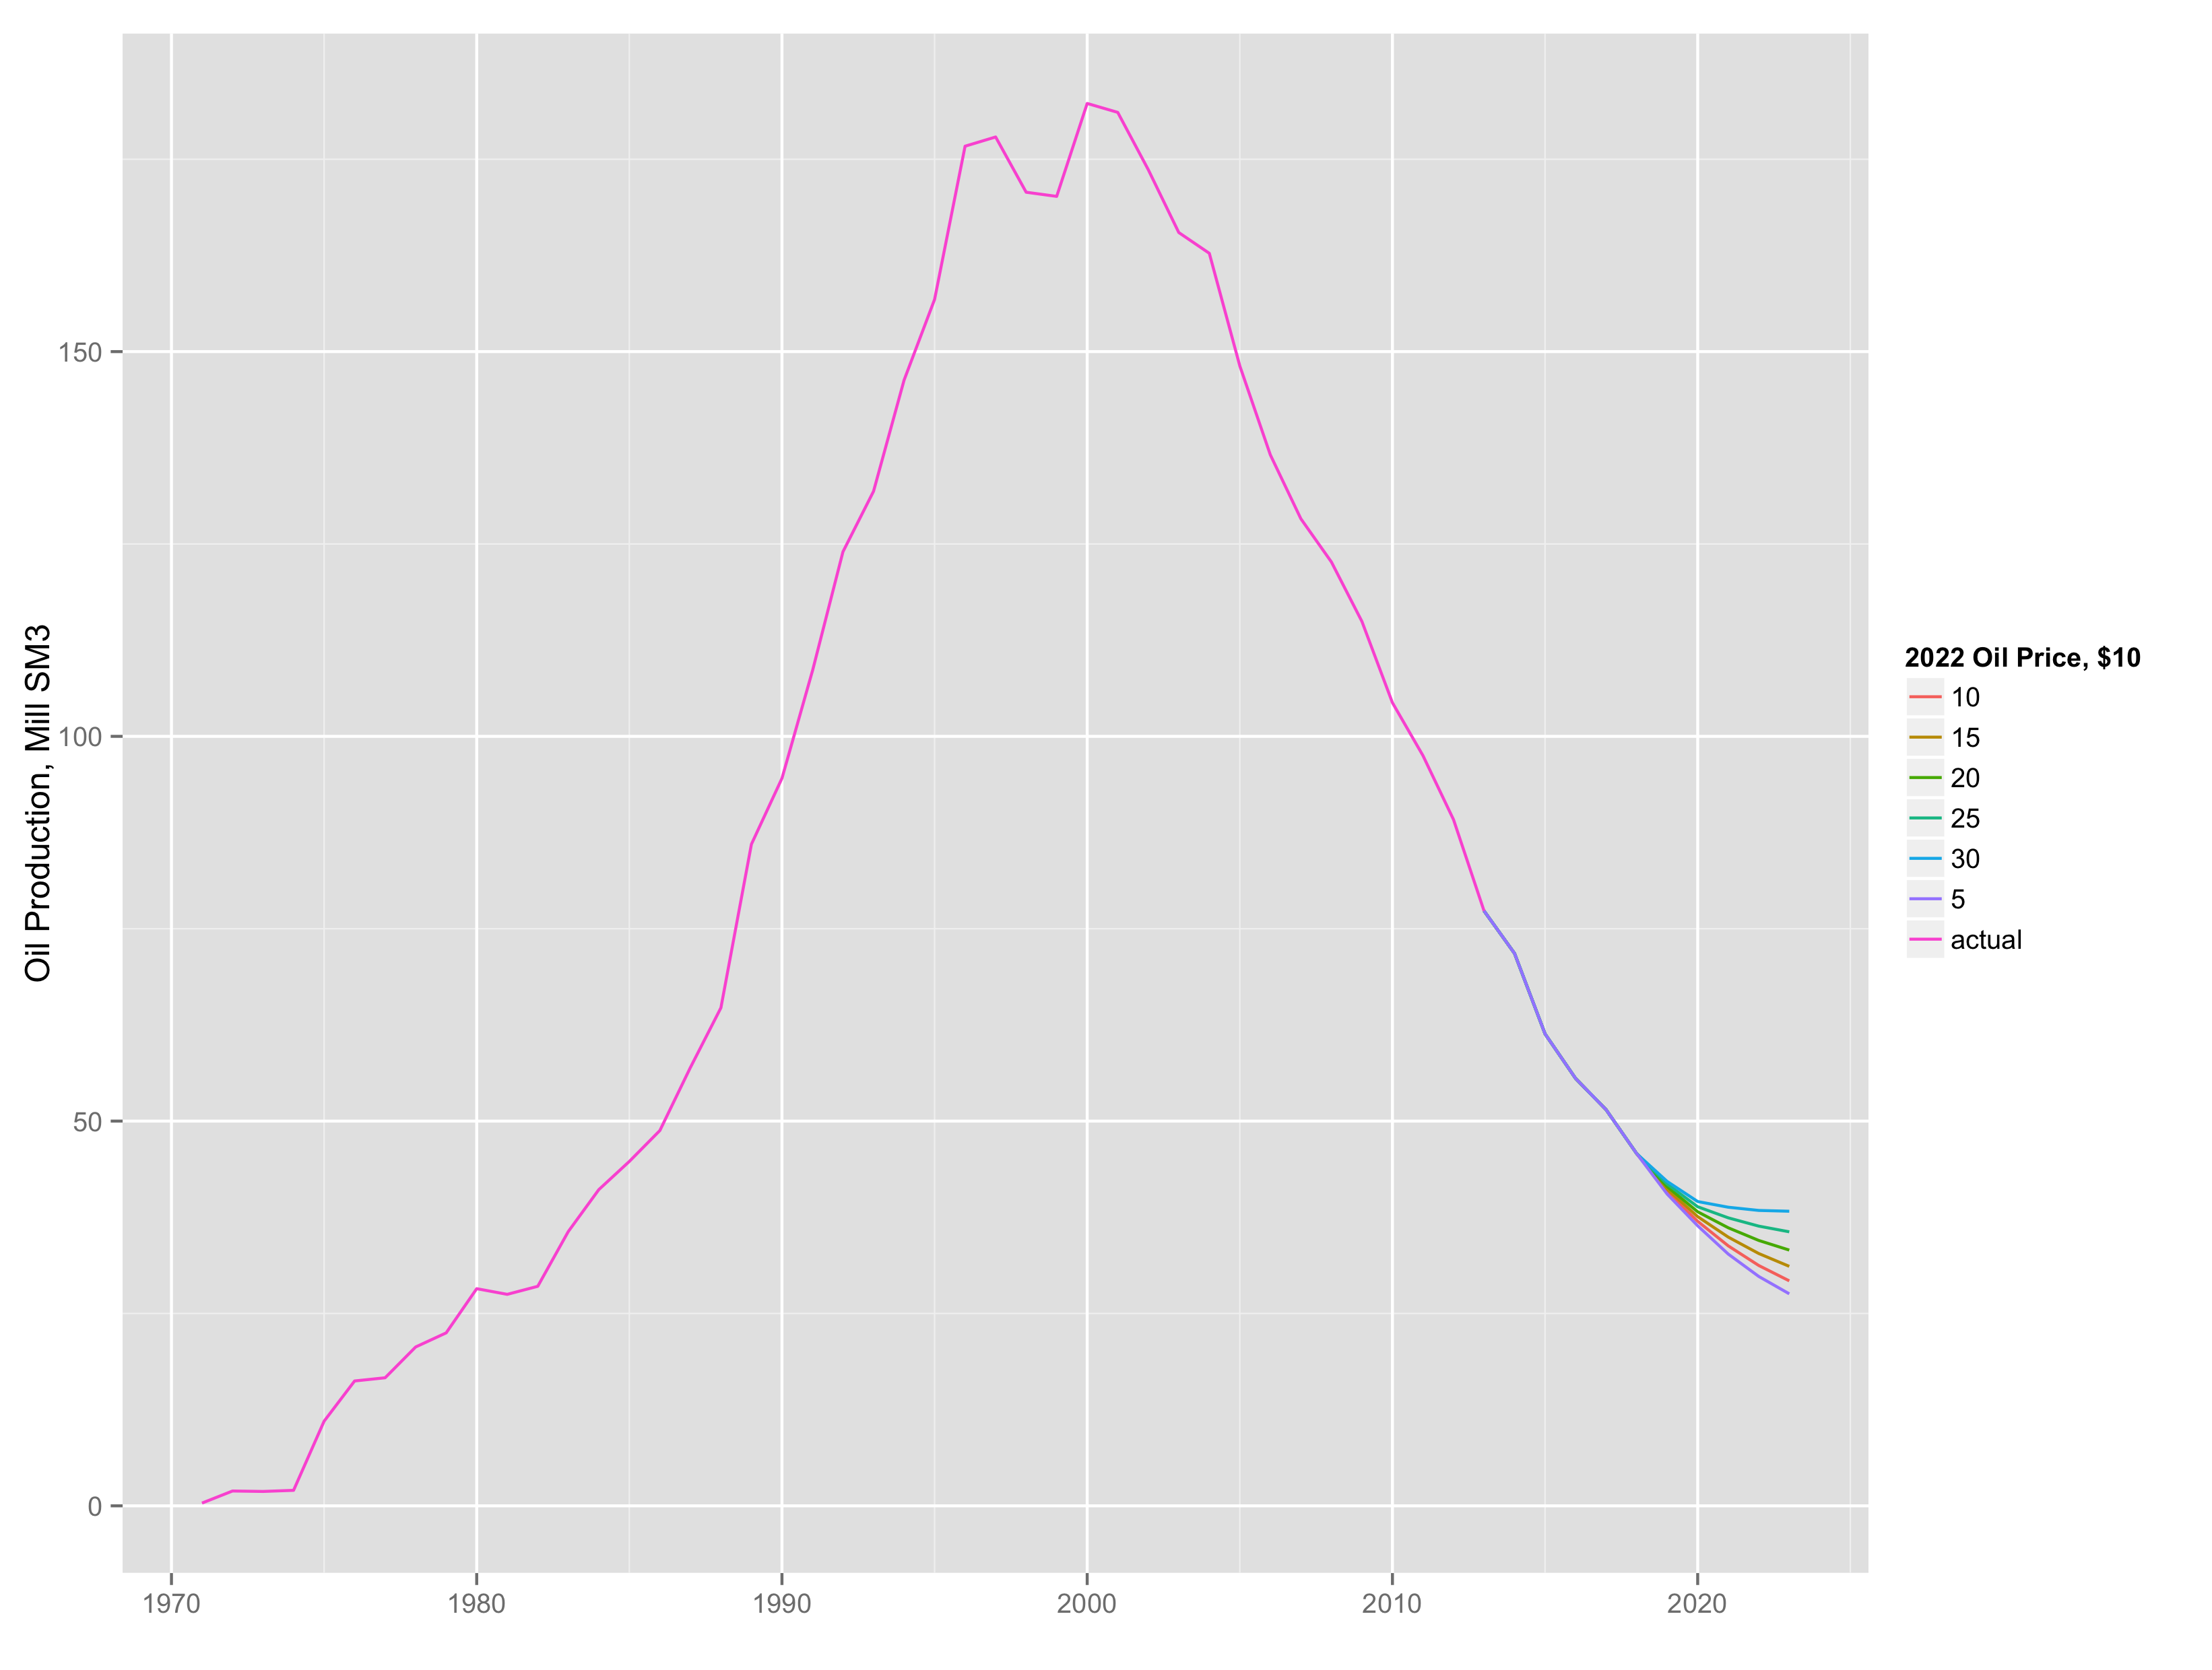
\includegraphics[width=.8\textwidth]{figures/tot_forecast.png}
		
		\label{tot_forecast}
	\end{figure}
\end{frame}

\begin{frame}[plain]
\begin{figure}
		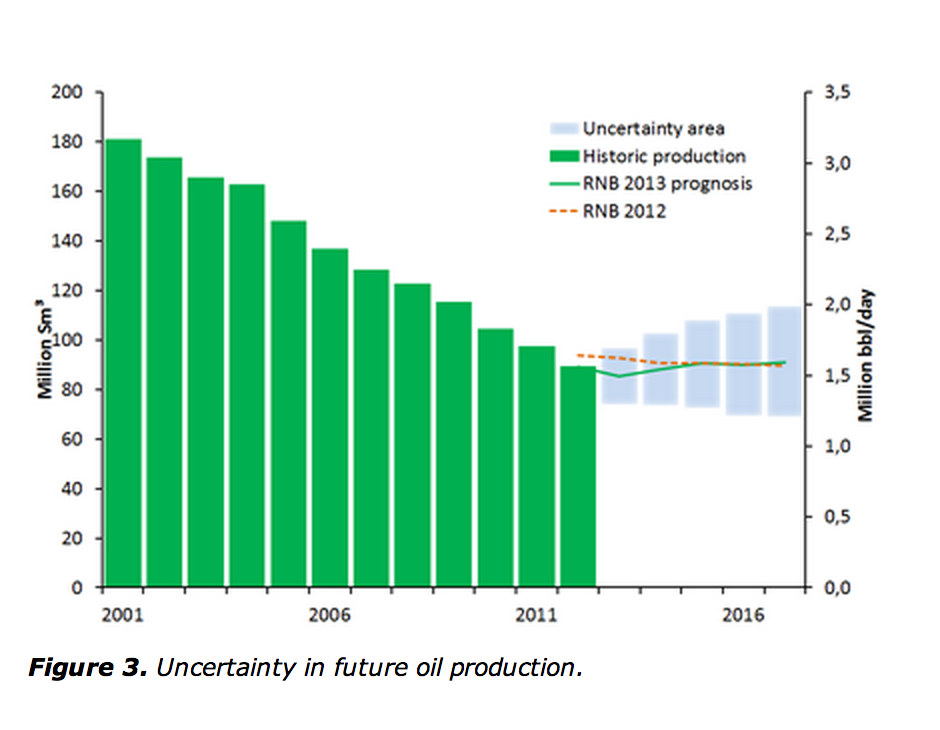
\includegraphics[width=.8\textwidth]{figures/NPD_oil_forecast.png}
		
		\label{NPD_oil_forecast}
	\end{figure}
\end{frame}

\end{document}